%!TEX root = ../report.tex
\chapter{Experiments and Results}
\label{chapter:experimentation_results}
The experiments focus on testing the different parts of the proposed strategy to configure a simulation instance provided by the user with optimal parameter configuration.
The final experiment, in section \ref{section:real_eval}, evaluates the cost and configuration response models in section \ref{section:training_phase} on unseen simulation instances. The models are compared using the runtime of the configurations predicted by the machine learning models against the best cost from SMAC. Owing to the unavailability of benchmarks for comparison, the comparison against the best cost from SMAC is used. In addition, the comparison against default configurations is avoided because default configurations practically result in crashed simulation for a few unseen simulation instances. The top three models are suggested to the user among the cost and configuration response models. In addition, the configuration predicted by the models is evaluated in terms of runtime against the default configurations on a critical simulation instance to illustrate the performance of the proposed strategy in figure \ref{fig:real_eval}.
The experiments are performed assuming the coupling tool MpCCI provides repeatable results for a particular configuration on a simulation instance. The experiments test the following aspects,
\begin{enumerate}
    \item Experiment 1: Performance comparison of SMAC best configuration and default configuration using the simulation runtime (in seconds).
    \item Experiment 2: Repeatability of SMAC to determine the optimal configuration for a particular simulation instance.
    \item Experiment 3: Number of iterations required to achieve reliable results by SMAC.
    \item Experiment 4: Ability of SMAC to find many good configurations for a particular simulation instance.
    \item Experiment 5: Performance comparison of the cost and configuration response models using RMSE across different data transformations to the cost metric discussed in section \ref{section:data_preprocessing}.
    \item Experiment 6: Evaluate the cost and configuration response models using the metrics in section \ref{section:evaluation_metrics} on unseen simulation instances to suggest the user with optimal configurations. 
\end{enumerate}


\section{SMAC best configuration versus default configuration}

The experimental setup section provides the simulation instances used in the experiment, solid and fluid solver coupled in MpCCI, the reason for experimenting, and the metrics used in this experiment. The results and discussion section compare the performance of SMAC best and MpCCI default configurations.

\subsection{Experimental setup}
This experiment illustrates the ability of SMAC to determine optimal configurations performing better than the default configuration. The experiment compares the runtime of the best configuration\footnote{Best configuration – This term is used with respect to SMAC. It is the configuration with the least runtime provided by SMAC for a particular instance.} from SMAC against the current default configuration provided in table \ref{table:parameterdefaultvalues} to perform simulation by experts.

The experiment is conducted on 16 different simulation instances. The features of the simulation instances are shown in table \ref{table:simulationinstances_train}. SMAC performs optimization for 100 iterations on each instance. Each iteration execute the target algorithm once. Calculix and OpenFOAM are the solid and fluid solvers respectively used for solving 3D driven cavity simulation problem. ABAQUS and OpenFOAM are the solid and fluid solvers respectively used for solving the elastic flap simulation problem. The best configuration for a particular simulation instance is the configuration with the least runtime among the 100 iterations. In this experiment, the mean percentage decrease in runtime and win percentage of SMAC are useful metrics to estimate the performance of SMAC best configuration against the default configuration. The mean percentage decrease in runtime is given by,
\begin{equation}
\text{Mean \% decrease in runtime } =
\frac{\text{Default cost}-  \text{SMAC best cost}}{\text{Default cost}} \times 100
\label{equation:decreasepercentage}
\end{equation}

The SMAC best cost and default cost is the simulation runtime on using the best configuration from SMAC and default configuration, respectively, expressed in seconds.

The win percentage of SMAC is the number of times SMAC best configuration perform better than the default configuration to the total simulation instances under optimization expressed as a fraction of 100. The performance is compared using the simulation runtime of a particular configuration. The matches is the 16 simulation instances under comparison.

\begin{equation}
\text{Win percentage} = \frac{\text{Number of wins}+ (0.5 \times \text{Number of draws})}{\text{Total number of matches}} \times 100
\label{equation:winpercentage}
\end{equation}

The win percentage in the above equation \ref{equation:winpercentage} provides the win percentage of SMAC.

% The number of wins is the number of times SMAC best configuration performance is better than the default configuration runtime. The number of draws is the number of times SMAC best configuration, and default configuration runtime are equal. The total number of matches is the simulation instances in the experimental set. In this experiment, the total number of instances is 16.

\subsection{Results and discussion}

The runtime of the best configuration from SMAC is compared against the runtime of the default configuration, as illustrated in table \ref{table:smac_vs_default}. The win percentage and mean percentage decrease in runtime is estimated.

\begin{table}[htbp]
\centering
\begin{tabular}{|c|c|c|c|}
\hline
\textbf{Instance} & \multicolumn{1}{|p{3.2cm}|}{\centering \textbf{Default configuration\\ cost (seconds)}}  & \multicolumn{1}{|p{3.2cm}|}{\centering \textbf{SMAC best configuration\\ cost (seconds)
}} & \multicolumn{1}{|p{3.2cm}|}{\centering \textbf{Decrease in runtime (percent)}}\\ \hline
1 & 447.84 & \color{blue}396.41 & 11.48 \\ \hline
2 & 505.66 & \color{blue}435.94 & 13.78 \\ \hline
3 & 609.80 & \color{blue}520.60 & 14.62 \\ \hline
4 & 435.58 & \color{blue}393.68 & 9.61 \\ \hline
5 & 673.68 & \color{blue}452.49 & 32.83 \\ \hline
6 & 2234.88 & \color{blue}2026.78 & 9.31 \\ \hline
7 & 2398.23 & \color{blue}1701.10 & 29.06 \\ \hline
8 & \color{red}Crashed & \color{blue}657.57 & NA \\ \hline
9 & \color{red}Crashed & \color{blue}569.00 & NA \\ \hline
10 & 1544.50 & \color{blue}1166.05 & 24.50\\ \hline
11 & 623.16 & \color{blue}513.217 & 17.64 \\ \hline
12 & 1184.54 & \color{blue}851.19 & 28.14 \\ \hline
13 & 3164.28 & \color{blue}2221.32 & 29.80 \\ \hline
14 & 1581.56 & \color{blue}344.37 & 78.22 \\ \hline
15 & \color{red}Crashed & \color{blue}1799.95 & NA \\ \hline
16 & \color{red}Crashed & \color{blue}1426.90 & NA \\ \hline
\end{tabular}
\captionsetup{justification=justified}
\caption[SMAC best configuration versus default configuration]{Comparison of SMAC best configuration versus default configuration.  The winner is highlighted in blue color text. The crashed simulations are highlighted in red and SMAC has optimized the instances.}
\label{table:smac_vs_default}
\end{table}

Owing to a very large cost value of the crashed simulations, the crashed default configurations are avoided for the mean decrease percentage calculation. The mean percentage decrease in runtime after optimization with SMAC is 24.92\% for a specific simulation instance. This metric provides an empirical estimate of SMAC performance in optimization tasks. 

\begin{table}[]
\centering
\begin{tabular}{|c|c|}
\hline
\textbf{Metric} & \textbf{Value} \\ \hline
Win percentage of SMAC & 100.00\% \\ \hline
Mean \% decrease in run-time & 24.92\% \\ \hline
\end{tabular}
\captionsetup{justification=justified}
\caption[Performance of SMAC best parameter configuration]{Performance comparison of SMAC best parameter configuration and default parameter configuration}
\label{table:experiment1_metrics}
\end{table}

SMAC has optimized all the crashed simulation instances efficiently as shown in table \ref{table:smac_vs_default}. This illustrates the efficiency of SMAC to find a better configuration even with bad initial configurations.

\section{Repeatability of SMAC }
\label{section:repeatability}

The experimental setup section provides the simulation instances used in the experiment, solid and fluid solver coupled in MpCCI, the reason for experimenting, and the metrics used in this experiment. The results and discussion section discuss the results of the experiment.

\subsection{Experimental setup}
Repeatability is the measure of variation between numerous measurements performed successively by an identical measurement procedure and conditions on the same subject within a short period of time \cite{repeatability1}. This experiment is performed to estimate the precision of SMAC in optimizing a particular simulation instance. In addition, this is a measure of the variance associated with the performance of a particular configuration provided by SMAC. For instance, a very high value of the repeatability coefficient indicates a large uncertainty associated with a particular configuration from SMAC. 

The experiment is conducted on 6 randomly selected simulation instances, namely, 1, 3, 4, 5, 6, and 12, provided in table \ref{table:simulationinstances_train}. The instances are optimized for 3 trials. SMAC performs optimization for 100 iterations for each trial. Calculix and OpenFOAM are the solid and fluid solvers respectively used for solving the simulation problem. The runtime of the best configurations from each trial is noted. This list of runtimes across 3 trials for a particular simulation instance is used to estimate the variance in the best runtime provided by SMAC. This variance is used to calculate the repeatability of SMAC.

\subsection{Results and discussion}

According to the repeatability co-efficient metrics provided in section \ref{section:repeatability_coeff}, the groups are the different simulation instances. The total mean ($\bar x_G$) is the average runtime of the best configuration from SMAC for all the instances under study. The mean run-time of each instance over 3 trials is $\bar x_k$ \cite{anova}. 

The sum of squared differences within each group ($SS_w $), represents the variability in the runtime of the best configurations from SMAC on a particular instance across the trials. $x_i$ is the value of a specific sample, $i$ in the group \cite{anova}. The within-group standard deviation is computed using LibreOffice Calc. The table \ref{table:smac_repeatability} provides the metrics computed.

\begin{table}[htbp]
\begin{center}
\begin{tabular}{|c|c|c|c|c|c|}
\hline
\multicolumn{ 1}{|c|}{\textbf{Instance}} & \multicolumn{3}{|p{4.5cm}|}{\centering \textbf{Best cost from\\ SMAC (seconds)}} & \multicolumn{1}{|p{2cm}|}{\centering \textbf{Average\\ cost (seconds)}}  & \multicolumn{1}{|p{2cm}|}{\centering \textbf{Standard\\ deviation\\(seconds)}}  \\ \cline{ 2- 4}
\multicolumn{ 1}{|c|}{} & \textbf{Trial 1} & \textbf{Trial 2} & \textbf{Trial 3} & \multicolumn{ 1}{l|}{} & \multicolumn{ 1}{l|}{} \\ \hline
1 & 399.84 & 397.82 & 396.41 & 398.02 & 1.72 \\ \hline
2 & 545.76 & 520.97 & 520.60 & 529.11 & 14.42 \\ \hline
3 & 403.16 & 393.68 & 416.12 & 404.32 & 11.26 \\ \hline
4 & 465.79 & 452.49 & 467.15 & 461.81 & 8.09 \\ \hline
5 & 2019.46 & 2026.78 & 2011.49 & 2019.24 & 7.64 \\ \hline
6 & 724.22 & 726.98 & 744.65 & 731.95 & 11.08 \\ \hline
\end{tabular}
\end{center}
\captionsetup{justification=justified}
\caption[SMAC mean runtime and standard deviation for different instances]{Average cost and standard deviation for the simulation instances involved in repeatability test of SMAC.}
\label{table:smac_repeatability}
\end{table}

% https://stats.stackexchange.com/questions/50727/f-statistic-f-critical-value-and-p-value

% \begin{figure}[!ht]
% \centering
% 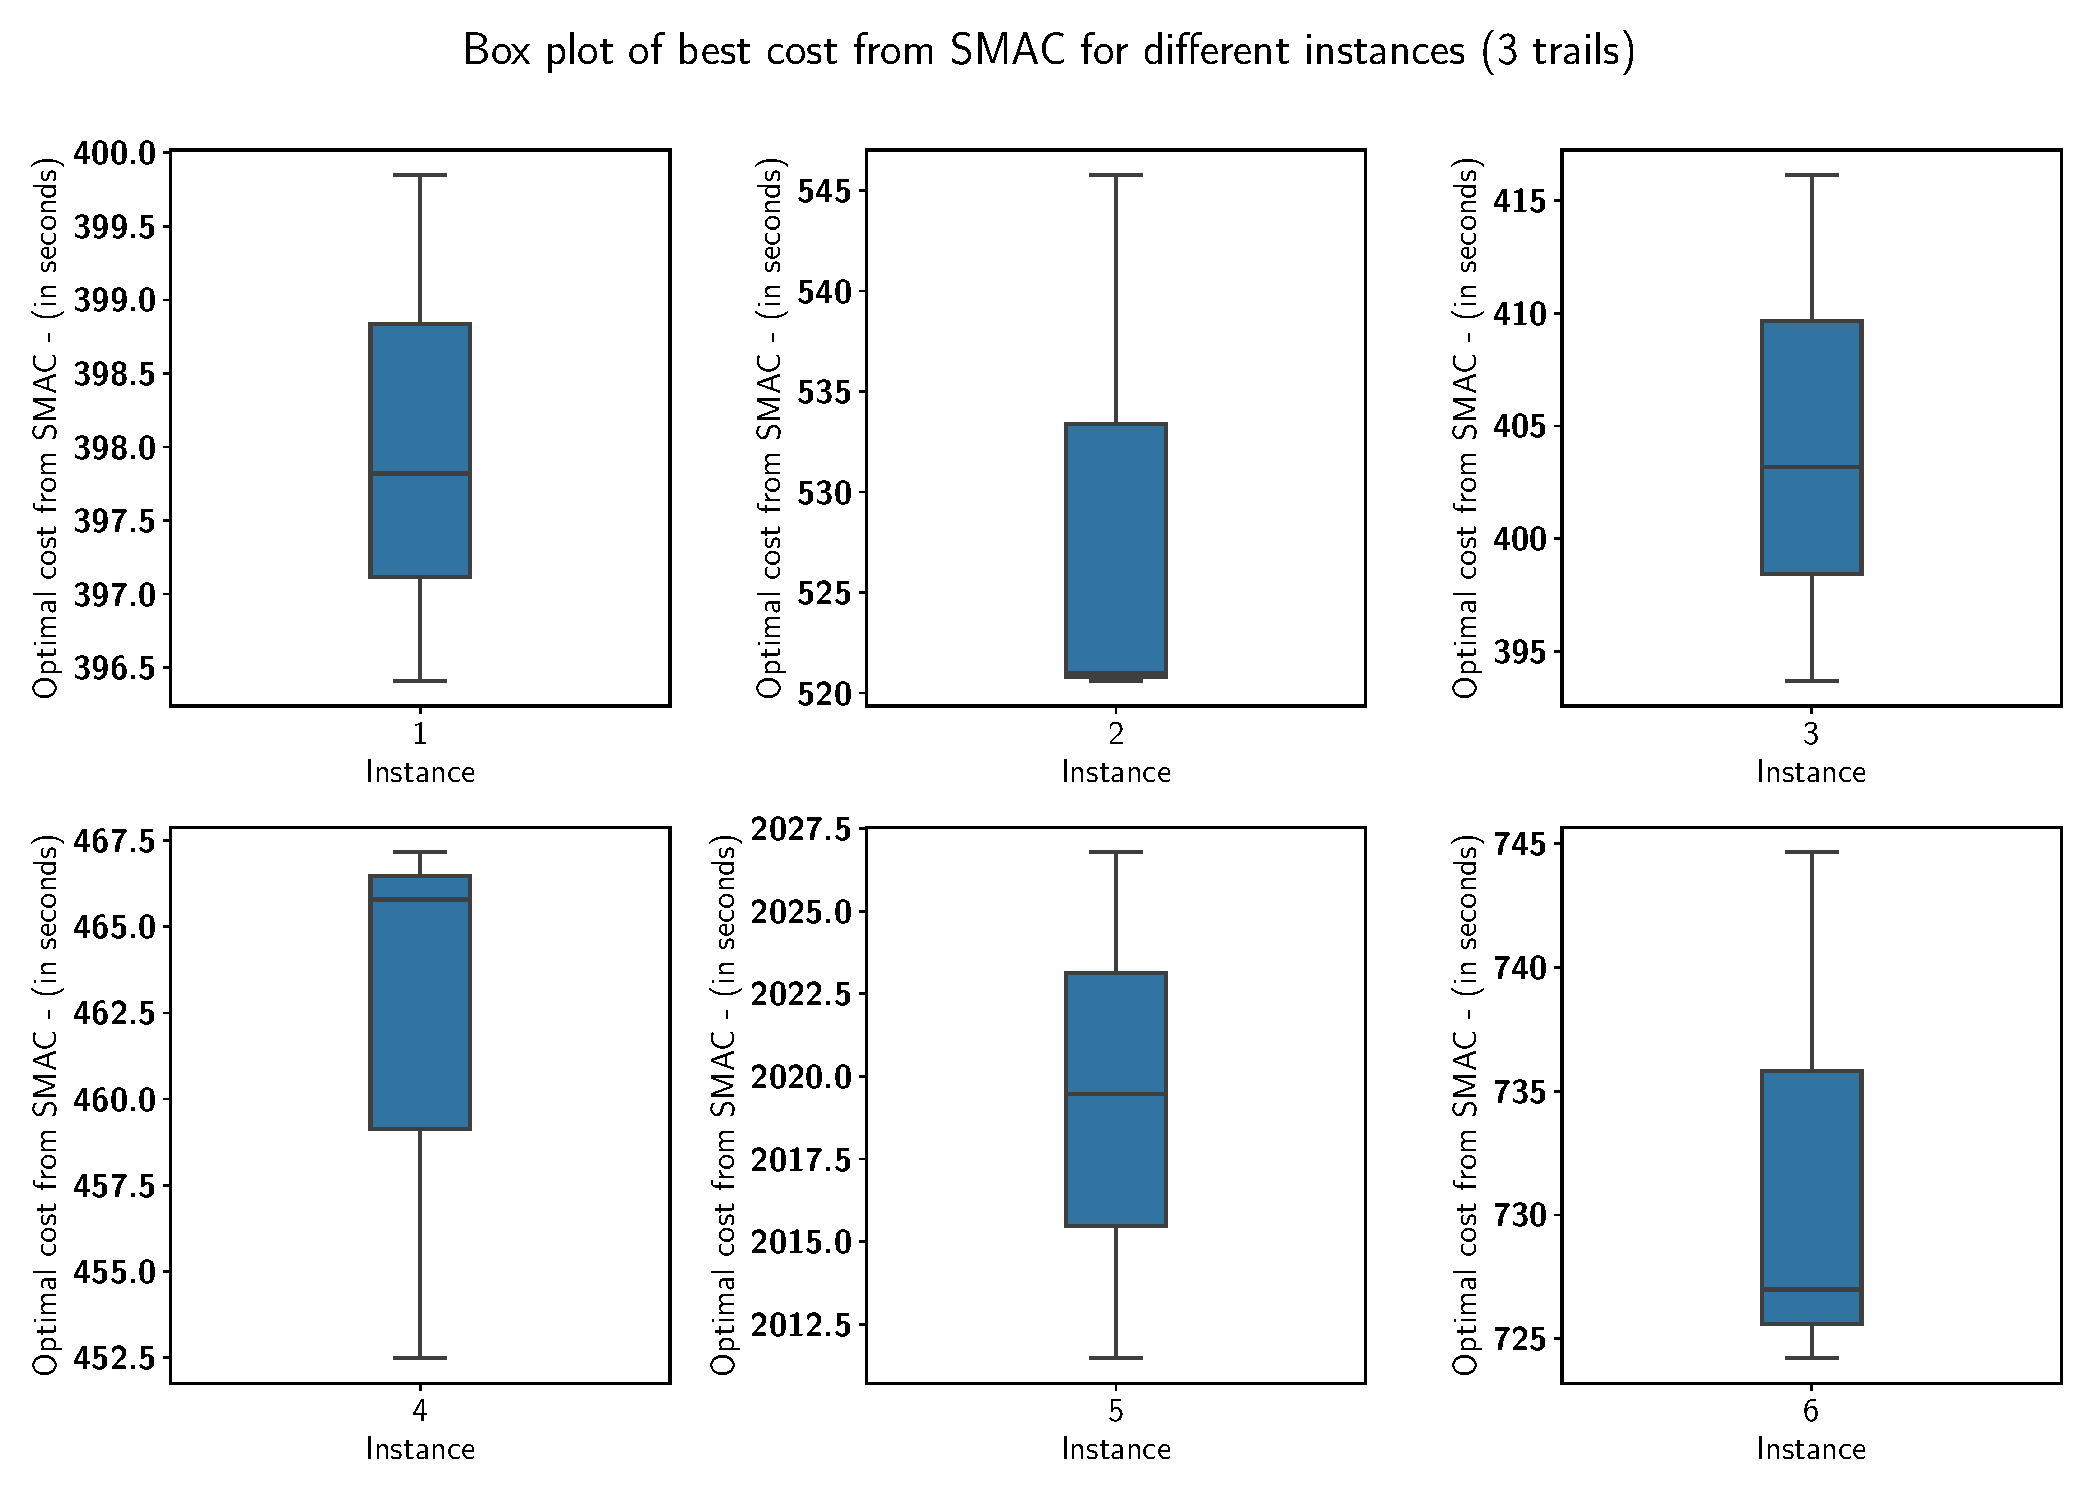
\includegraphics[width=\textwidth]{images/SMAC_repeat_boxplot.pdf}
% \captionsetup{justification=justified}
% \caption[Box plot of SMAC best configuration for different instances]{Box plot for the SMAC best configuration for the 6 random instances of the experimental set of instances. 3 trails is performed for each instance.}
% \label{fig:boxplots_repeatability}
% \end{figure}


\begin{table}[!h]
\centering
\begin{tabular}{|c|c|}
\hline
\textbf{Metric} & \textbf{Value} \\ \hline
\begin{tabular}[l]{c@{}l@{}}Mean variation in run-time within\\ simulation instances $(MS_w)$\end{tabular} & 97.46 seconds \\ \hline
Repeatability coefficient $(S_r)$ & 19.34 seconds \\ \hline
\end{tabular}
\captionsetup{justification=justified}
\caption[SMAC repeatability metrics]{SMAC repeatability metrics}
\label{table:experiment3_metrics}
\end{table}

Therefore, with a probability of 95\%, the maximum difference in runtime between two successive best configurations from SMAC on the same simulation instance under the same conditions is 19.34 seconds. 


\section{Behavior of SMAC with respect to iteration count}

The simulation instances used in the experiment and the reason for performing the experiment is provided in the experimental setup. In addition, the experimental procedure is breifly provided. The results and discussion section discuss the results of the experiment.

\subsection{Experimental setup}

The reason for performing the experiment is to identify the optimal number of iterations required to estimate relatively lesser runtime by SMAC on a particular simulation instance. In addition, the experiment provides an estimation of the number of target algorithm runs SMAC performs to identify optimal configurations.

The experiment is conducted only on 4 different, randomly selected instances. In addition, the random selection is restricted to simulations performing more iterations in a lesser amount of time. The simulation instances 3, 4, 5, 8, and 12 are selected. The features of the instances are provided in table \ref{table:simulationinstances_train}. Each simulation instance is optimized by SMAC for an iteration count of 300. The best configuration is estimated at 6 checkpoints of iterations, namely 25, 50, 100, 150, 200, 250, and 300.

\subsection{Results and discussion}

The graphs in figure \ref{fig:experiment3_results} illustrates the performance of SMAC to find better configurations with reduced runtime. SMAC successfully finds better configurations on increasing iterations. However, the problem in executing SMAC for substantial iterations is the target algorithm is executed for each iteration. Therefore, the many iterations of SMAC are practically challenging to execute. In addition, the figure \ref{fig:experiment3_results} illustrates a saturation behavior of SMAC to find better configuration compared to the initial iterations.

\begin{table}[!h]
\centering
\begin{tabular}{|c|c|c|c|c|c|c|c|}
\hline
\multirow{2}{*}{\textbf{Instance}} & \multicolumn{7}{c|}{\textbf{Best cost (seconds) for different SMAC iteration (itr) count}} \\ \cline{2-8} 
 & \textbf{25 itr} & \textbf{50 itr} & \textbf{100 itr} & \textbf{150 itr} & \textbf{200 itr} & \textbf{250 itr} & \textbf{300 itr} \\ \hline
1 & 528.41 & 528.41 & 520.97 & 520.97 & 520.97 & 520.97 & 520.97 \\ \hline
2 & 410.08 & 397.13 & 397.13 & 393.68 & 393.68 & 393.68 & 393.68 \\ \hline
3 & 733.68 & 521.01 & 479.41 & 470.28 & 466.56 & 456.33 & 456.33 \\ \hline
4 & 905.96 & 768.97 & 735.53 & 735.53 & 726.98 & 726.98 & 726.98 \\ \hline
\end{tabular}
\captionsetup{justification=justified}
\caption[Performance of SMAC best configuration versus iteration count]{Best cost (run-time in seconds) from SMAC for different iteration counts of 4 randomly selected simulation instances.}
\label{table:experiment3_results}
\end{table}

\begin{figure}[!h]
\centering
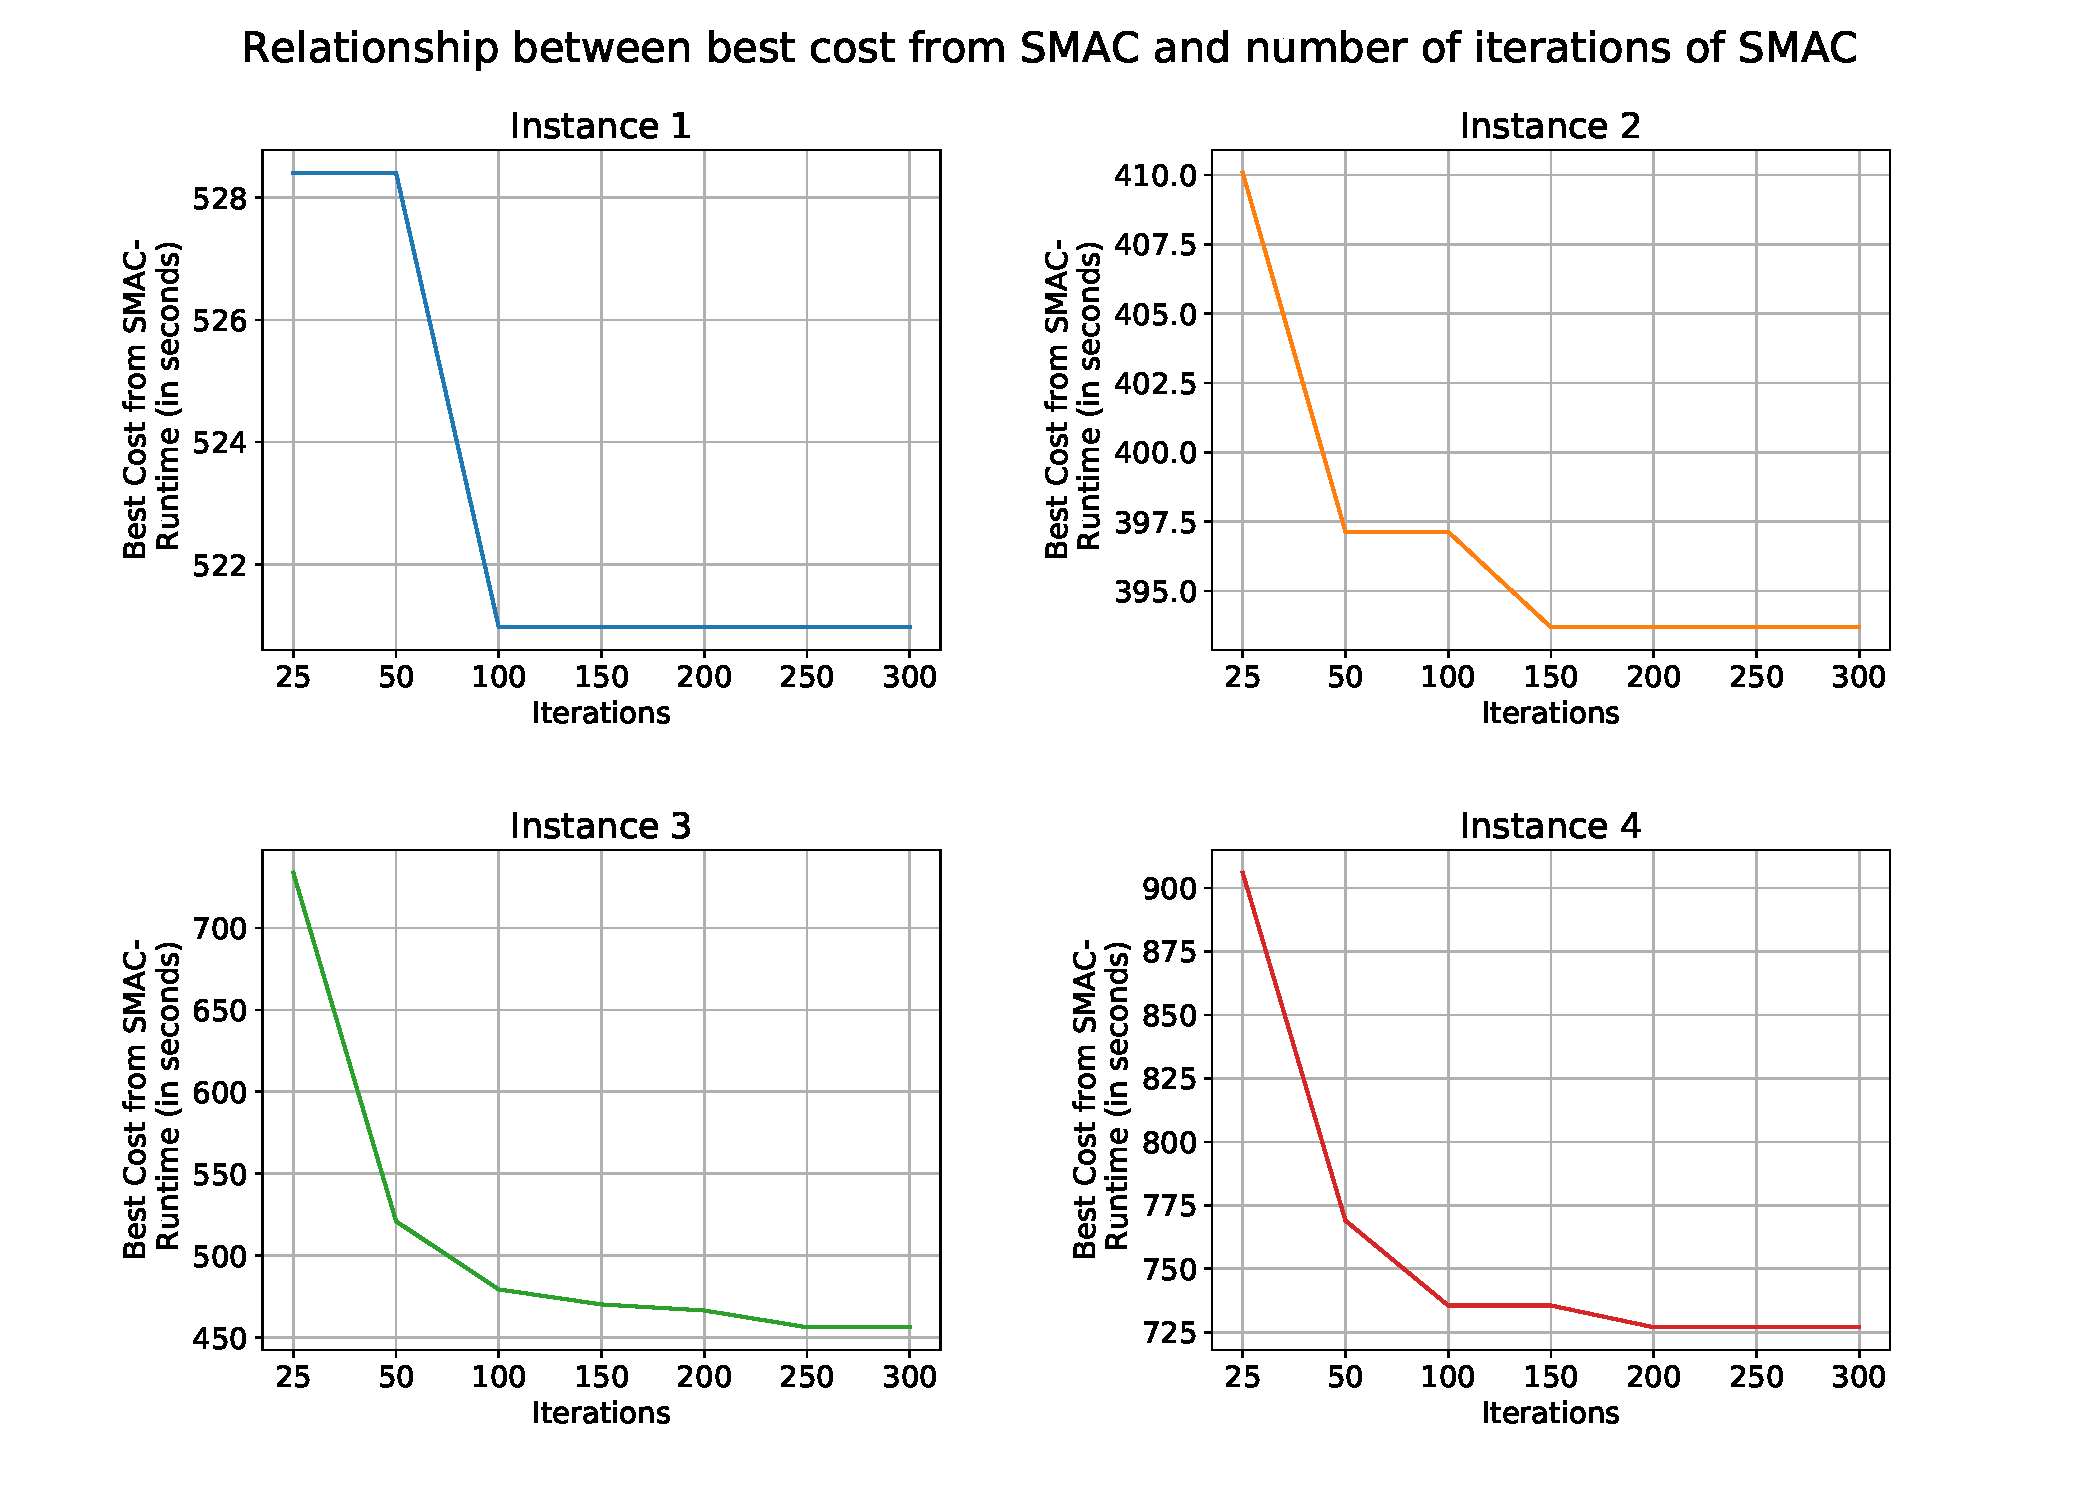
\includegraphics[width=\textwidth]{images/Iteration_vs_cost.pdf}
\captionsetup{justification=justified}
\caption[An illustration of SMAC best cost versus iteration count]{SMAC best cost versus number of iterations. The ability to find good configurations increases with iteration count.}
\label{fig:experiment3_results}
\end{figure}

\section{SMAC Good-Bad-Ugly configurations}

The previous experiments focus on the quality of the good parameter configurations obtained by SMAC on optimizing a single instance. This section analyses the search trajectory of SMAC and aid in selecting the training data from the dataset generated.

% The section provides an analysis of the quality of search performed by SMAC over the 100 iterations to optimize a single instance. 

\subsection{Experimental setup}
This experiment provides a deeper insight into the run history of SMAC and analyzes the search path of SMAC. SMAC keeps track of all the parameters configurations $\theta_i$ and the respective cost metric $c_i$ on evaluating a particular simulation instance $\pi_i$ \cite{CAVE_paper}. This set of parameters configurations, simulation instances, and respective cost metric is called run history, r = $\{\theta_i, \pi_i, c_i,\}_{i=1}^N$, N is the number of iterations of SMAC for optimizing a particular instance. In this research, the instances are optimized for 100 iterations. The run history of the 16 instances provided in table \ref{table:simulationinstances_train} is utilized. 

\begin{figure}[!ht]
\centering
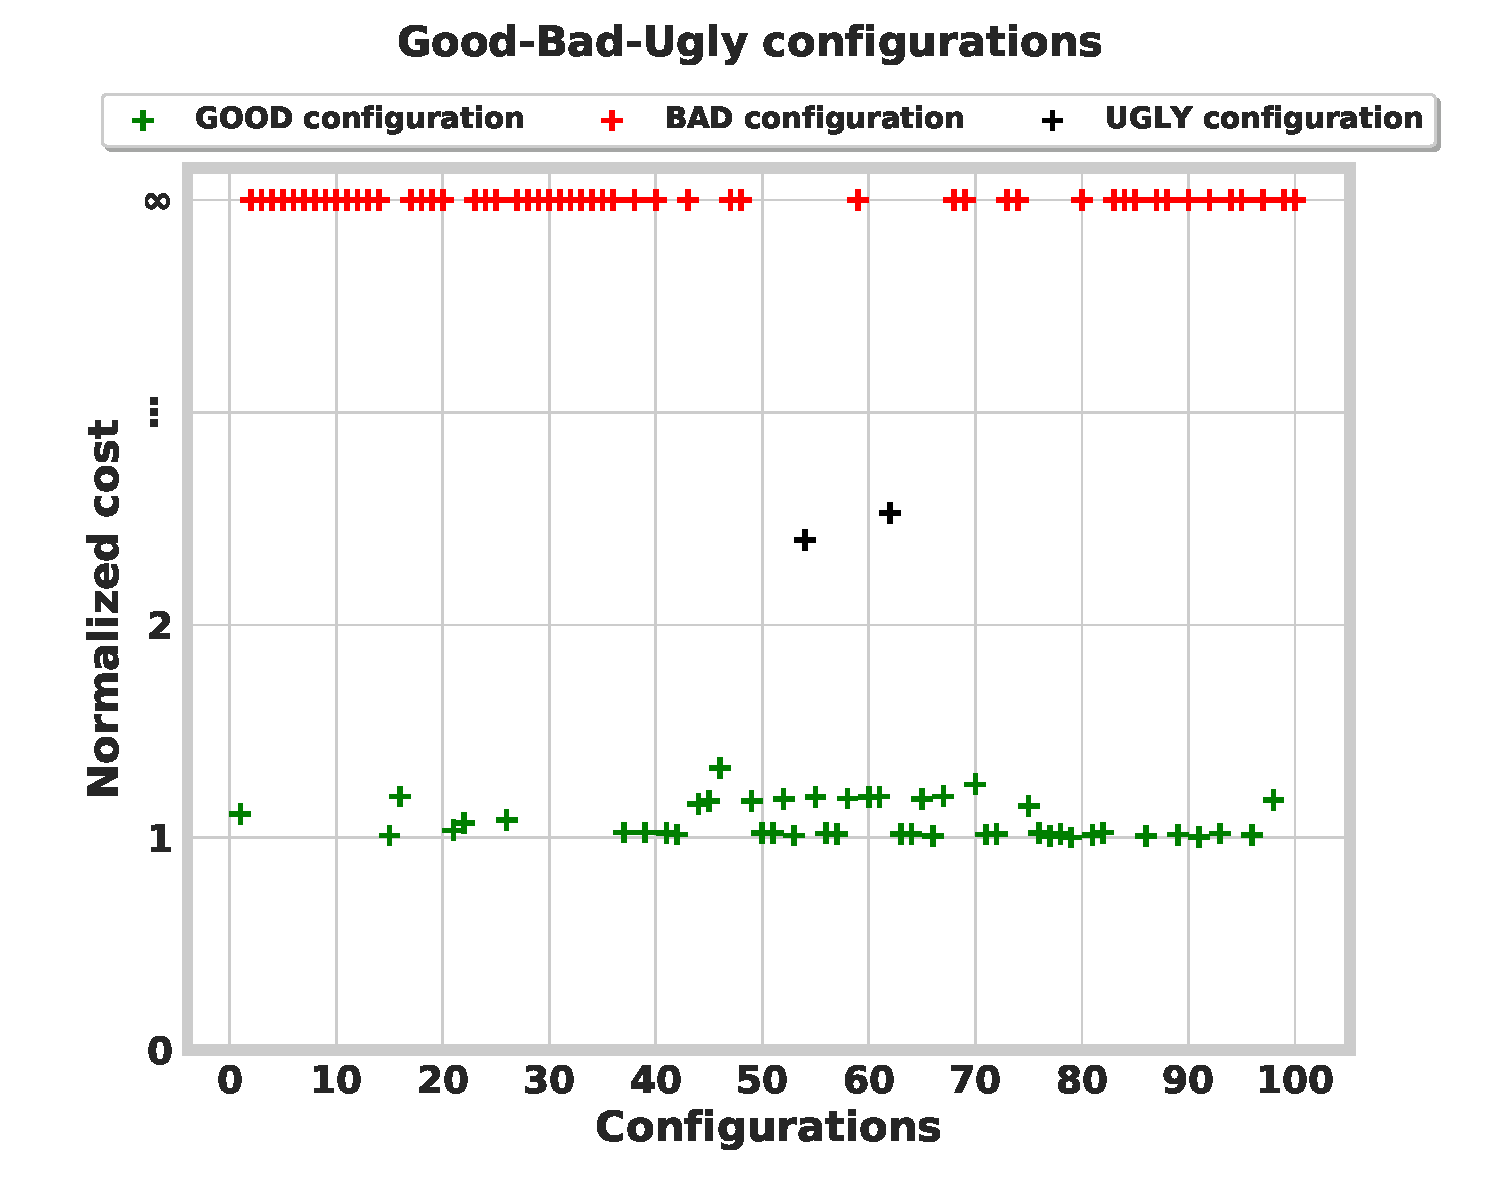
\includegraphics[width=0.85\textwidth]{images/Good_bad_ugly_cost.pdf}
\captionsetup{justification=justified}
\caption[An illustration of good-bad-ugly configurations from SMAC]{An illustration of good-bad-ugly configurations for single instance optimization over 100 iteration. Each iteration is performed with a different parameter configuration. Good and ugly configurations result in successful simulation. Bad configurations result in crashed simulation. The cost metric (runtime in seconds) has been normalized with the best cost from SMAC for a particular simulation instance.}
\label{fig:good-bad-ugly}
\end{figure}


% The following section \ref{section:good-bad-ugly-metrics} provides an explanation of the good, bad, and ugly configurations to analyze the run history of SMAC in optimizing the multiphysics simulations.

The configurations resulting in crashed simulations are bad configurations (red markings in figure \ref{fig:good-bad-ugly}). The configurations resulting in a successful simulation (green and black markings in figure \ref{fig:good-bad-ugly}) for a particular instance are sub-divided into good (green) and ugly (black) configurations depending on the cost metric associated with the configuration. The good configurations are the sub-optimal configurations performing close to the best cost of SMAC. The ugly configurations are the configurations performing below a particular threshold relative to the sub-optimal configurations. For instance, in figure \ref{fig:good-bad-ugly} for illustration purposes, the threshold is set to be the normalized cost values above the upper inner fence (Q3 + 1.5 $\times$ IQR) \cite{outlier} normalized cost value of the distribution of the successful simulation. Interquartile Range (IQR) is the difference between third (Q3, $75^{th}$ percentile) and first quartile (Q1, $25^{th}$ percentile), (IQR = Q3-Q1).

However, the exact value of the threshold of cost for configurations performing lesser than sub-optimal configurations for FSI multiphysics simulations should be explored in the future. The plot in figure \ref{fig:good-bad-ugly} represents the distribution of normalized cost over 100 iterations of SMAC for a single simulation instance.

% Best cost in SMAC is the optimal cost. 
% Near best cost in SMAC is the sub-optimal.
% Below sub-optimal is ugly.

%  Defense point -> why cant you remove the outliers and work on green configs only?
%  Because practically there may be some cases where the data in good and ugly are distributed widely where the many good configs are relatively far away from the best cost biasing the model similar to the bad configs. So it is important to find the threshold that works over the complete dataset or FSI simulations for a feature set. Like OOD data for a simulation instance. Currently, therefore the entire successful simulation has been used.



% \begin{figure}[!h]
%         \centering
%         \begin{subfigure}{.48\textwidth}
%               \centering
%               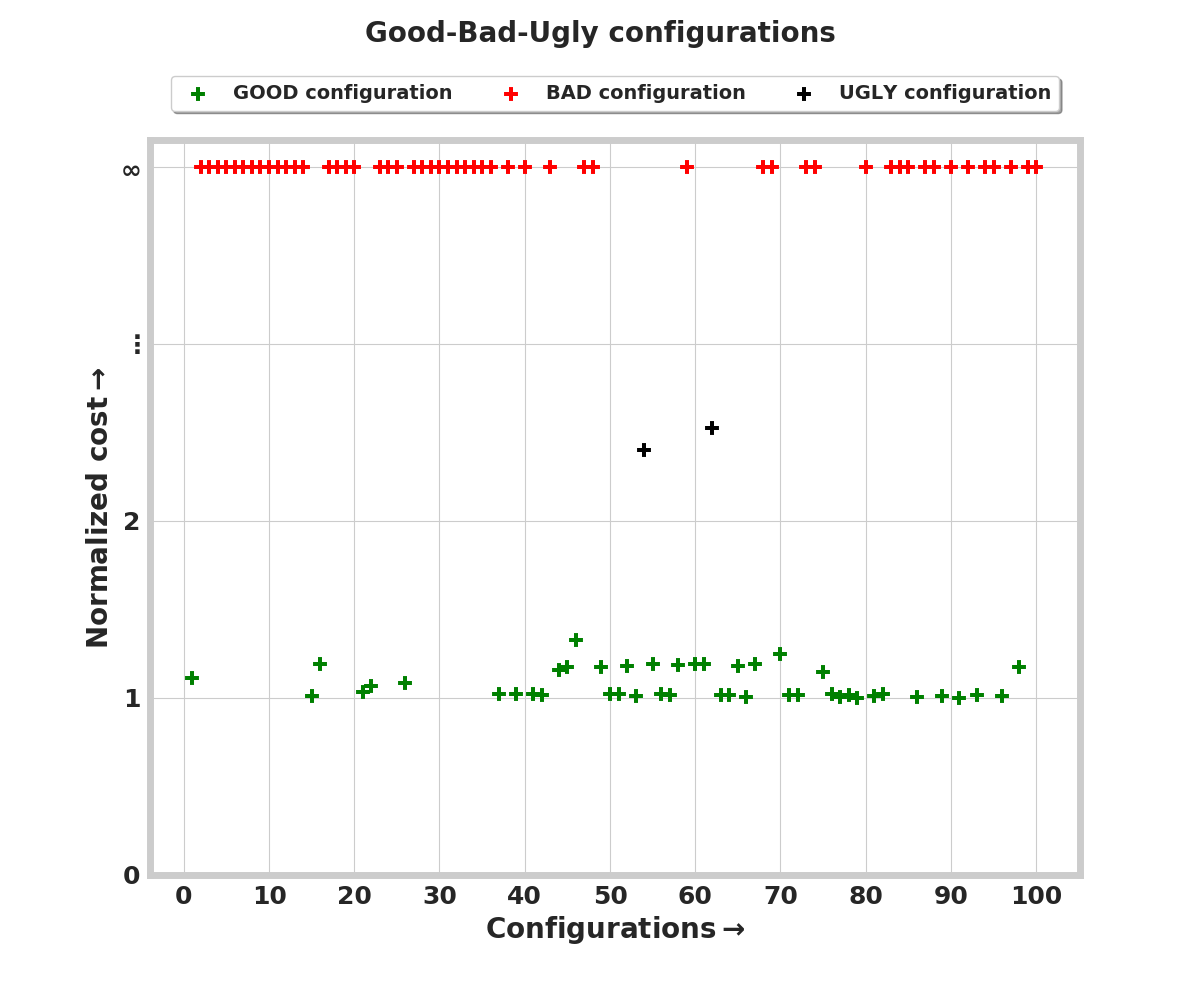
\includegraphics[width=1\linewidth, height=0.3\textheight]{images/Good_bad_ugly_cost.png}
%               \caption{Good-Bad-Ugly configurations.}
%               \label{fig:good-bad-ugly}
%         \end{subfigure}
%         \begin{subfigure}{.48\textwidth}
%               \centering
%               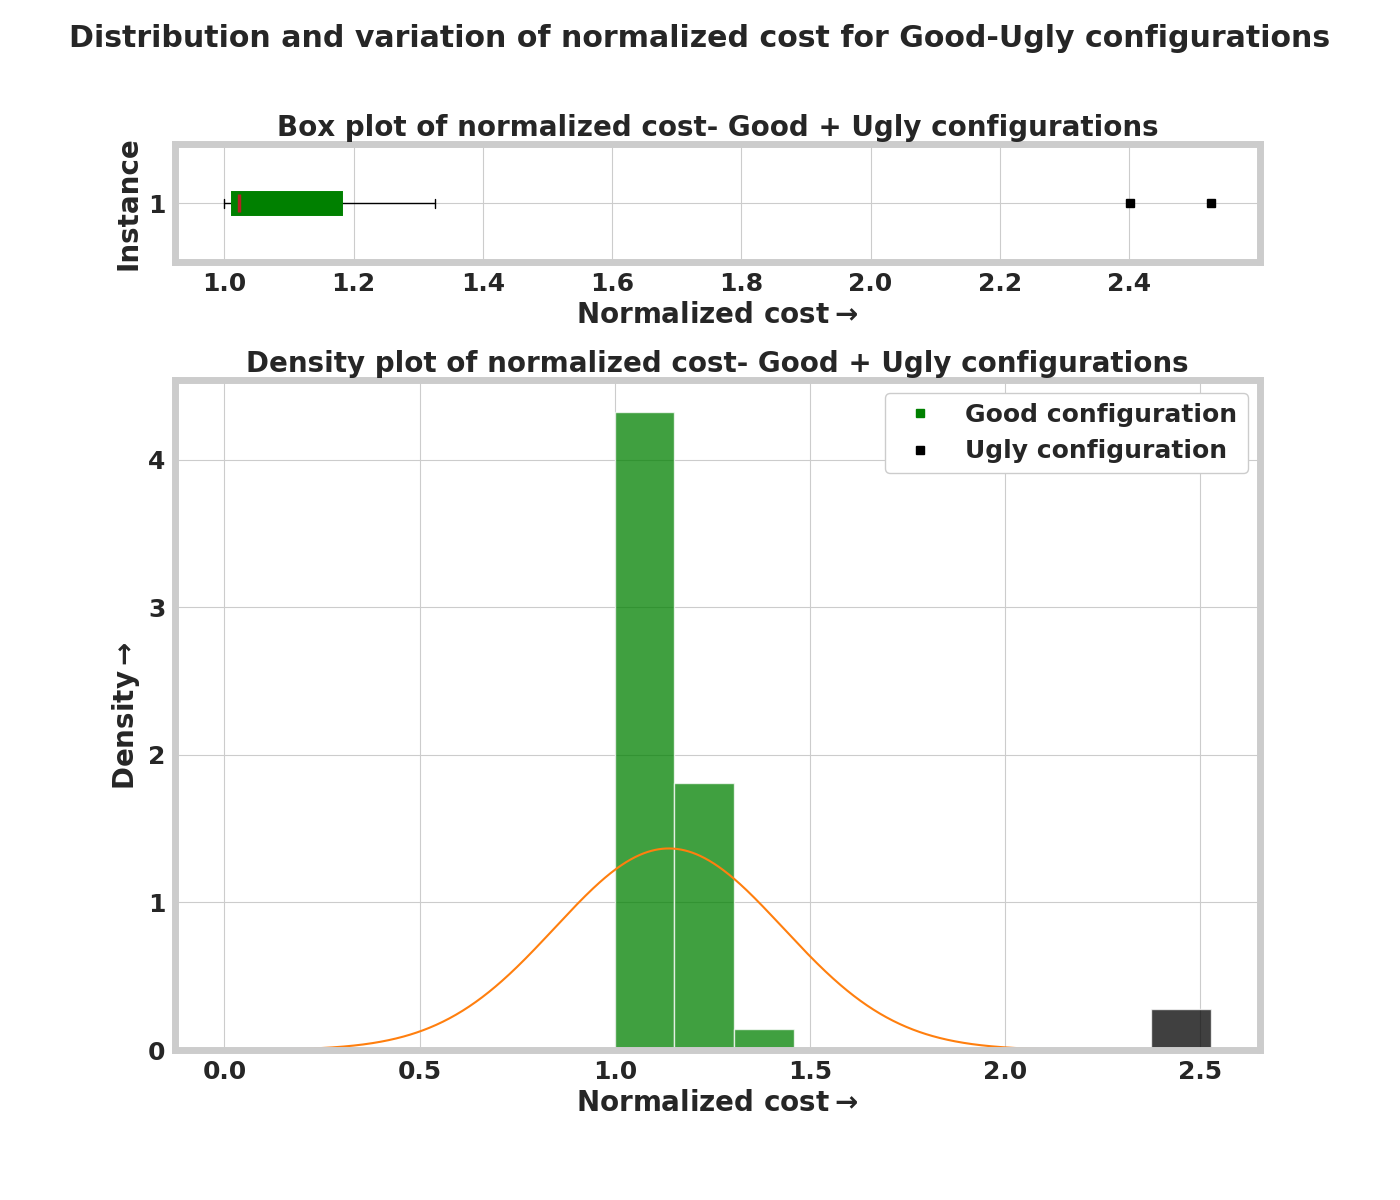
\includegraphics[width=1\linewidth, height=0.32\textheight]{images/Good_ugly_dist.png}
%               \caption{Distribution of good and ugly configurations.}
%               \label{fig:good-ugly}
%         \end{subfigure}
% \caption{An illustration of good-bad-ugly configurations. Good and ugly configurations result in successful simulation. Bad configurations result in crashed simulation.}
% \label{fig:good-bad-ugly}
% \end{figure}

Good configurations percentage, bad configuration percentage, and ugly configuration percentage are the number of good, bad, and ugly configurations present in 100 iterations of the SMAC for a particular instance. 

\subsection{Results and discussion}

On calculating the average good, bad, and ugly configurations percentage across all the 16 instances, the good and bad percentage is approximately close. The table \ref{table:configuration_split} provides the percentage of good-bad and ugly configurations.

\begin{table}[!ht]
\centering
\begin{tabular}{|c|c|}
\hline
\textbf{Configurations} & \textbf{\% of total configurations} \\ \hline
The Good (Optimal and sub-optimal) & 49.2 \\ \hline
The Bad (Crashed) & 47.8 \\ \hline
The Ugly (Below sub-optimal) & 3.0 \\ \hline
\end{tabular}
\captionsetup{justification=justified}
\caption[Percentage of good-bad-ugly configurations from SMAC]{Percentage of good-bad-ugly configurations from SMAC for per-instance optimization (average over 16 instances). The ugly configurations are considered to be the configurations with normalized cost value above the upper inner fence (Q3 + 1.5 $\times$ IQR) of the successful simulations distribution.}
\label{table:configuration_split}
\end{table}

The interest of this research work is to predict configurations resulting in successful simulation. The bad configurations bias the predictions by the regressor towards crashed simulation configurations. Therefore, the bad configurations are removed in the data pre-processing step. However, the threshold for defining ugly configurations is a future work of the research.

% Bad configurations increase the variance in the data, and the model would not learn the good also properly.
% Having all successful is also not so good because it can also have large variance luckily in our case there are no such large variances. We have to find optimal configurations near the best cost of SMAC.
% In addition, reducing the number of bad configurations aid in reducing the number of target algorithm evaluations. The additional evaluations over-utilize the resources in terms of memory, time, and license of utilizing the solid-fluid solvers. 

% This increases the need to run SMAC with a larger good configuration percentage. Therefore, one recommendation is pruning SMAC after searching for a particular number of bad configurations. The next section focuses on training a classification model to detect good (successful) simulations and bad (crashed) simulations for pruning SMAC using the good and bad configurations available in the dataset.

% \section{Classification model to prune SMAC}

% The reason for developing the classification model to classify successfully and crashed simulations is insightful from the previous experiment. This section focuses on providing an overview of the data processing steps from the dataset generated in the optimization phase, training procedure, evaluation metrics for model selection, and performance of the different models in the classification of successful and crashed simulations.
% \subsection{Experimental setup}

% The dataset from optimization phase includes the following features,

% \begin{enumerate}
%     \item Parameter configurations, $\theta_i$.
%     \item Features of the simulation instance $f_i$.
%     \item Cost, $c_i$ of evaluating the parameter configuration $\theta_i$ in the simulation instance with features $f_i$.
% \end{enumerate}

% The crashed simulations are provided a huge cost (2147483647.0) by SMAC, symbolizing the not defined ($\infty$) cost of a crashed simulation. The crashed simulations are provided a labeled, 1, positive, and the successful simulations are labeled, 0, negative in the study. The features of the simulation instance and parameters are the features of the training set. The reason is the features and parameters are only the information available before the execution of each instance. The number of observations in the dataset is 1600.

% A vector representation of the dataset is created using the label or ordinal encoding for the categorical variables. The classifiers- Logistic regression, K-Nearest Neighbors (KNN), Random Forest (RF), Gradient boosting, and Support Vector Machine (SVM) are selected for preliminary analysis. K-Fold cross-validation (CV) is the model selection method used with a split count five (5-Fold CV).

% The best parameters of each model are identified using hyperparameters tuning. The hyperparameters of each model are tuned for best parameters using the GridSearchCV API available in scikit-learn \cite{scikit-learn} \cite{sklearn_api}. The metrics accuracy, precision, recall, and F1 score are used to compare the model performance.

% \subsection{Results and discussion}

% The PCA and t-SNE plots in figure \ref{fig:pca} and \ref{fig:tsne} aid visualizing the high dimensional feature space of successful and crashed simulation features in a lower dimension.

% % PCA axis represents the variance in components 1 and 2.
% % t-SNE axis does not mean anything because it is just the mapping of high dimension to low dimension. The relative distance between points in low dimension. Even after normalizing the high dimension, the points are highly varied in the graph.

% \begin{figure}[!h]
%         \centering
%         \begin{subfigure}{.48\textwidth}
%               \centering
%               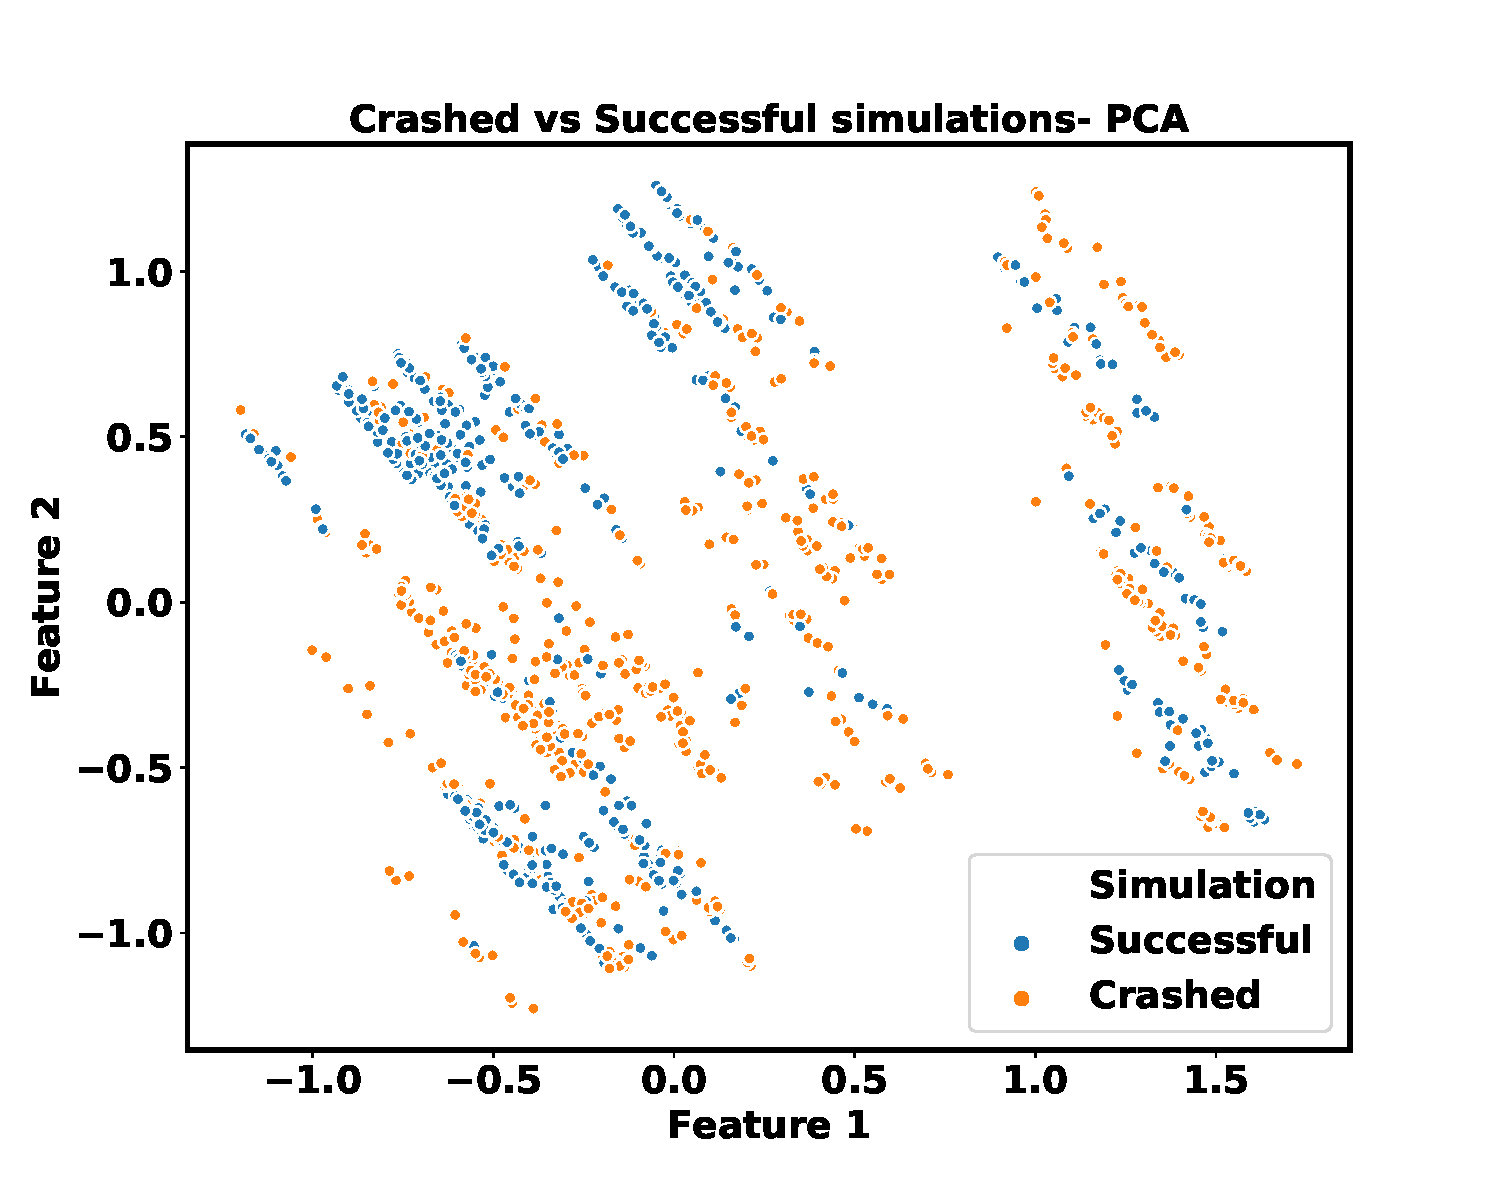
\includegraphics[width=\textwidth]{images/pca.pdf}
%               \caption{PCA}
%               \label{fig:pca}
%         \end{subfigure}
%         \begin{subfigure}{.48\textwidth}
%               \centering
%               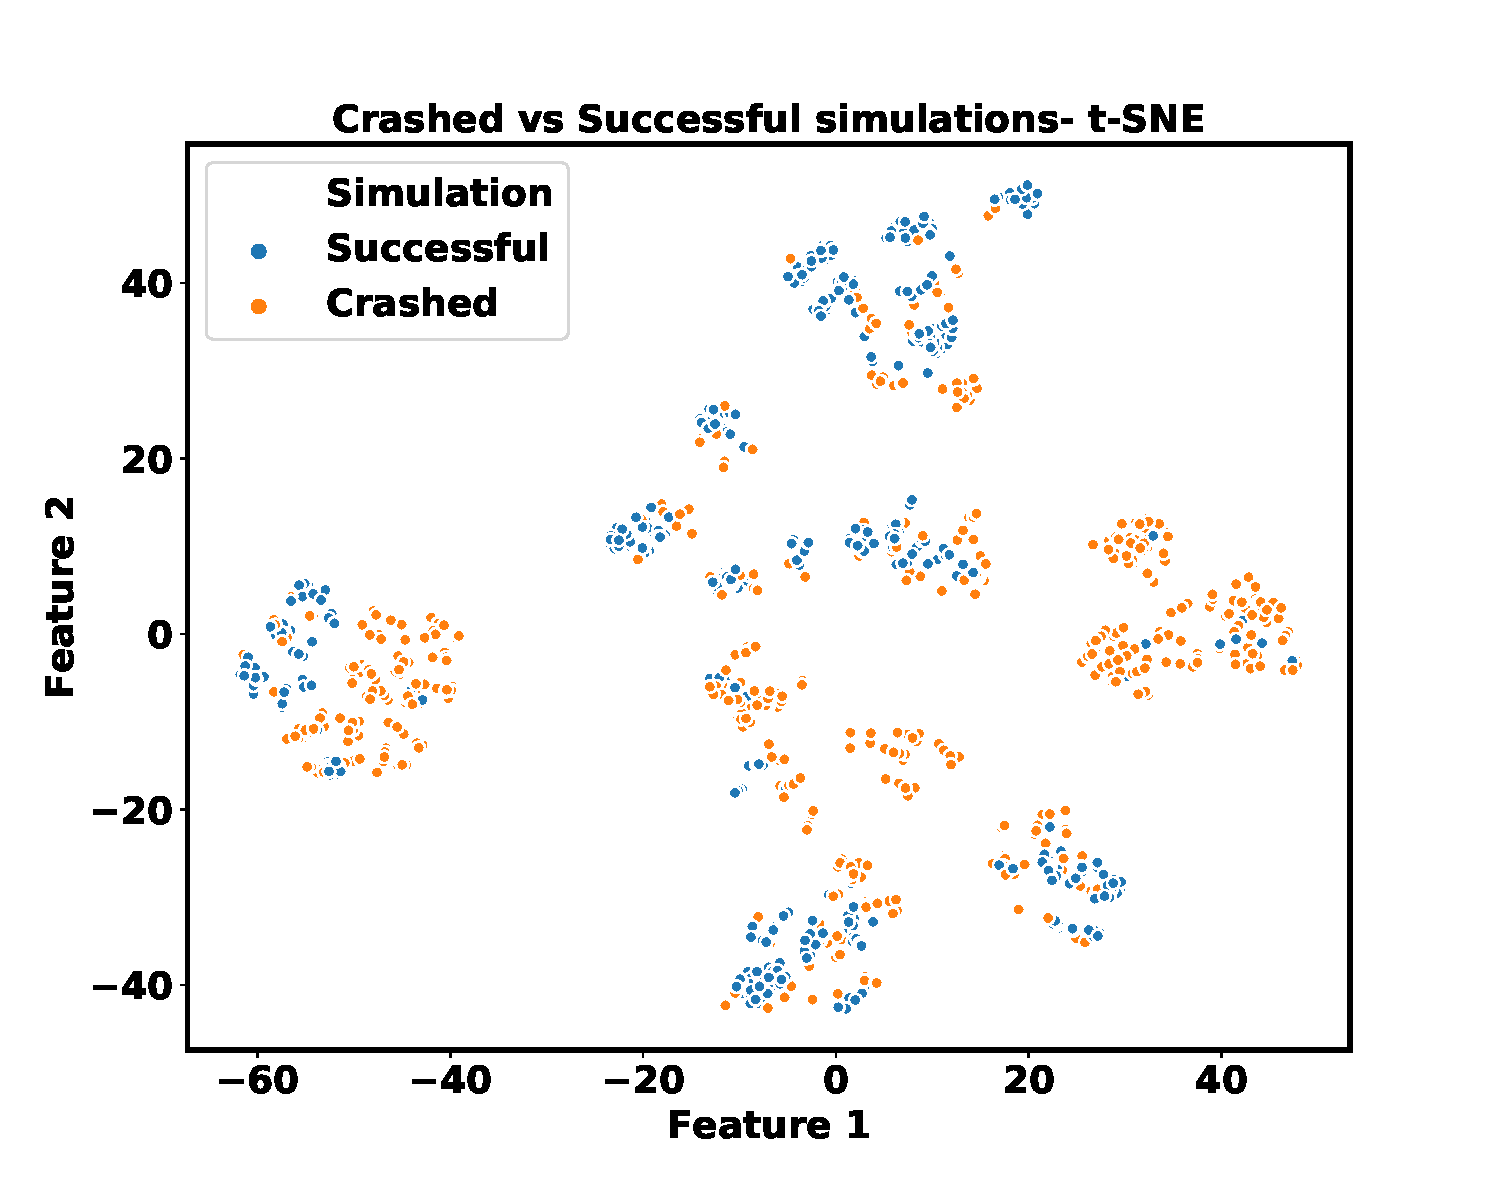
\includegraphics[width=\textwidth]{images/tsne.pdf}
%               \caption{t-SNE}
%               \label{fig:tsne}
%         \end{subfigure}
% \caption[PCA and t-SNE plot for successful and crashed simulations]{PCA and t-SNE with 2 features of successful and crashed simulations. The distribution of simulation types based on the features of the training set illustrate the simulation types are not easily separable.}
% \label{fig:PCAandtsne}
% \end{figure}

% % The parameters of each model are optimized using 5-fold cross-validation following a parameter grid provided by the user in a grid search. The values of the model, in contrast to the default values, are provided below.

% % \begin{enumerate}
% %     \item Logistic regression: C = 1, class weight = balanced.
% %     \item Random forest: number of trees = 100, maximum depth of the tree = 3.
% %     \item Support Vector Machine: C = 10, gamma = 1, kernel = 'rbf'.
% %     \item K-nearest neighbors: number of neighbors,K = 10.
% %     \item Gradient boosting: number of trees = 40. 
% % \end{enumerate}

% On performing 5-fold CV on the dataset, the results obtained are provided in the table \ref{table:classificationresults}. The blue markings indicate the best performing model performance. The SVM with radial basis function (RBF) with regularization parameter C=1 and $\gamma$=0.1 kernel outperforms other classifiers in all metrics.

% % The figure \ref{fig:SVM-confusionmatrix} illustrates a the confusion matrix of SVM generated by 5-fold CV. The confusion matrix is generated by summing each test set confusion matrix of 5-folds CV \cite{confusionmatrix-CV} \cite{confusionmatrix-CV-stackoverflow} \cite{Matlab-confusionmatrix}. Therefore, the total observations is equal to the total observations in the dataset.

% % Gradient boosting outperforms logistic regression, KNN, and SVM because of the various categorical variables available in the dataset. The reason GBM performs better than RF is because of the less bias in the model because of the weak classifier used in GBM.

% \begin{table}[]
% \centering
% \begin{tabular}{|l|l|l|l|l|}
% \hline
% \begin{tabular}[c]{@{}l@{}}\textbf{Model} \\\end{tabular}  & \begin{tabular}[c]{@{}l@{}}\textbf{Accuracy} \\\textbf{(\%)} \end{tabular}& \begin{tabular}[c]{@{}l@{}}\textbf{Precision} \\\textbf{(\%)} \end{tabular} & \begin{tabular}[c]{@{}l@{}}\textbf{Recall} \\\textbf{(\%)}\end{tabular} & \begin{tabular}[c]{@{}l@{}}\textbf{F1 score} \\\textbf{(\%)} \end{tabular} \\ \hline
% \begin{tabular}[c]{@{}l@{}}Logistic regression \\ \end{tabular} & 82.14 & 84.60 & 76.29 & 80.21 \\ \hline
% \begin{tabular}[c]{@{}l@{}}Random forest\\ (100 trees)\end{tabular} & 86.04 & 88.09 & 81.63 & 84.72 \\ \hline
% \begin{tabular}[c]{@{}l@{}}\color{blue}Support Vector\\\color{blue}  Machine (RBF kernel)\end{tabular} & \color{blue}96.81 & \color{blue}98.17 &\color{blue} 95.31 &\color{blue}  96.71 \\ \hline
% \begin{tabular}[c]{@{}l@{}}K-Nearest Neighbors\\ (k=10)\end{tabular} & 89.46 & 95.61 & 81.54 & 88.01 \\ \hline
% \begin{tabular}[c]{@{}l@{}}Gradient boosting\\ (40 trees)\end{tabular} & 92.38 & 92.72 & 88.87 & 90.74 \\ \hline
% \end{tabular}
% \captionsetup{justification=justified}
% \caption[Successful and crashed simulations classifier performance]{Classification results of successful and crashed simulations. The metrics are obtained by 5-Fold cross-validation. The blue markings indicate the best model selected.}
% \label{table:classificationresults}
% \end{table}

% \begin{figure}[!ht]
% \centering
% 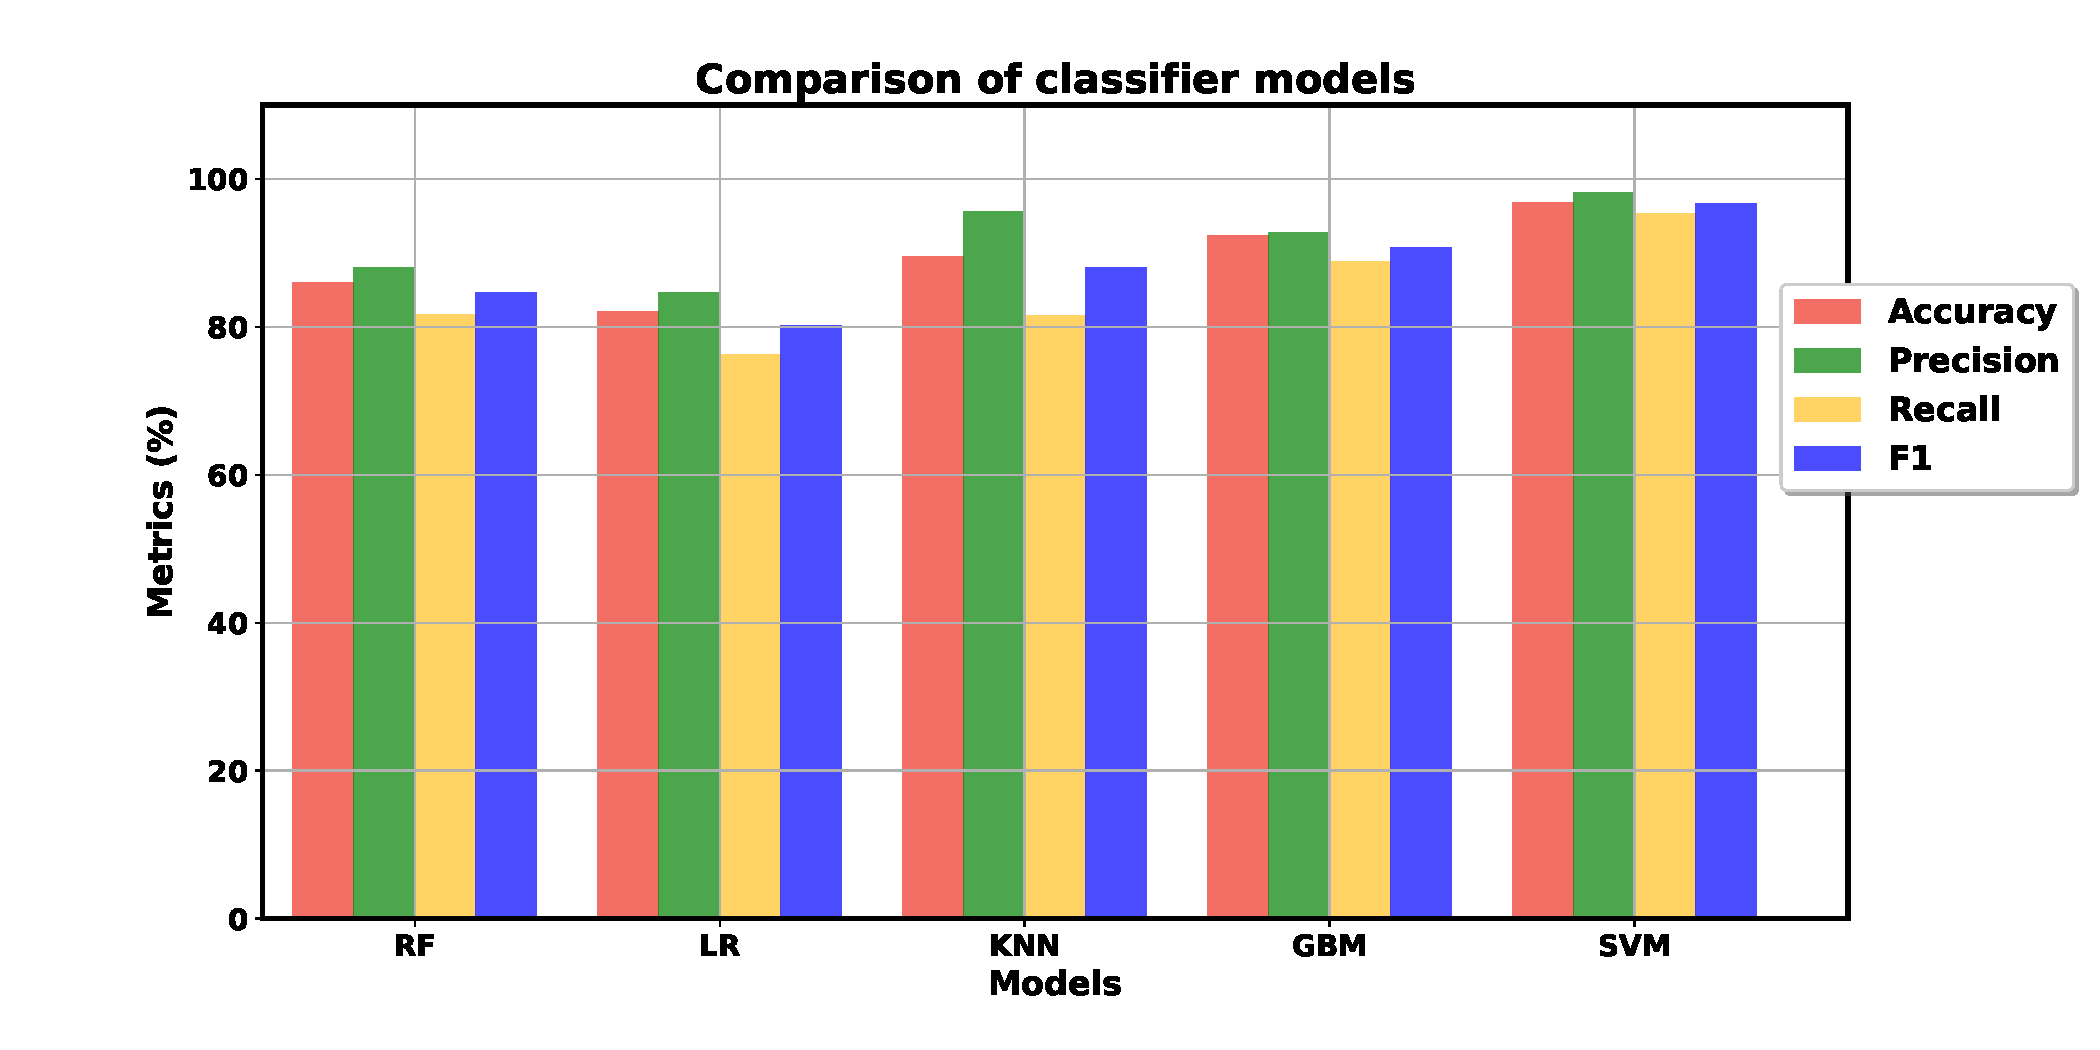
\includegraphics[width=\textwidth]{images/classificationmetrics.pdf}
% \caption[Successful and crashed simulations classifier performance]{Illustration of model performance by 5-fold CV. SVM outperforms other models in successful versus crashed simulation.}
% \label{fig:classificationmetrics}
% \end{figure}

% % \begin{figure}[!ht]
% % \centering
% % 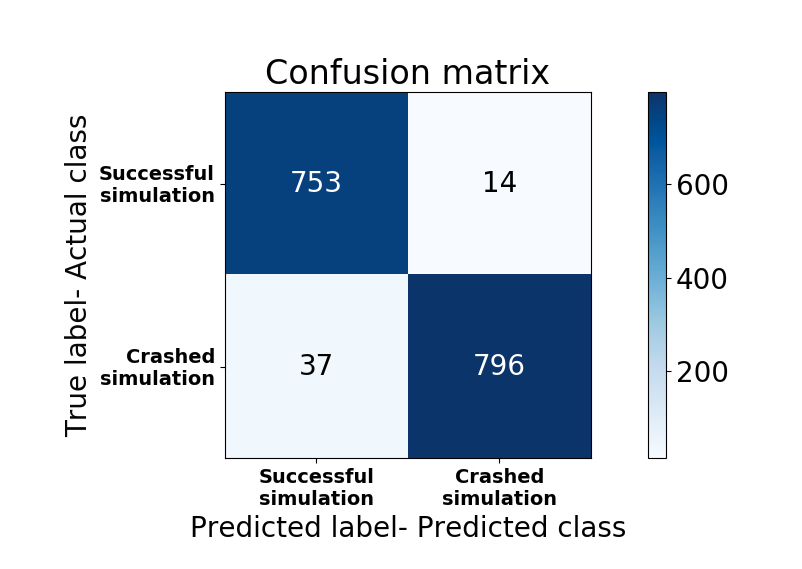
\includegraphics[width=0.9\linewidth,height=0.4\textheight]{images/SVM-confusionmatrix.png}
% % \caption[Confusion matrix of SVM- Successful versus crashed simulations]{Confusion matrix of SVM classifier by 5-fold CV.}
% % \label{fig:SVM-confusionmatrix}
% % \end{figure}

% Therefore, a suggestion to improve the good configuration percentage and reduce the crashed simulation in the run history of SMAC is to use SVM to classify successful and crashed simulations. SVM with RBF kernel is suggested for pruning SMAC in between the 100 iterations. In pruning, the algorithm is forced to proceed with the next iteration by selecting new challenger configurations and challenge the current best configuration. However, this is one of the suggested methods to prune SMAC for multiphysics simulations. 

% The graph in figure \ref{fig:gradientboostingvalid} illustrates the accuracy of GBM for the various number of trees by 5-fold cross-validation. The difference between the train and validation accuracy is very low for 40 trees providing an excellent fit for the data.

% https://stats.stackexchange.com/questions/173390/gradient-boosting-tree-vs-random-forest - Useful for pitch

\section{Comparison of model performances and runtime transformations}
\label{section:trainingexperiment}
The following experimental setup section provides an overview of the instances and machine learning models used in the experiment. In addition, procedure to train the models is explained. The results and discussion section provides the comparison of model performance using RMSE. The models are trained using data with different transformations applied to the cost metric (runtime in seconds) feature.

\subsection{Experimental setup}

This experiment compares the performance of the cost and configuration response models in predicting the optimal configuration for a given simulation instance. The models are trained on the dataset created by optimizing 16 instances provided in the table \ref{table:simulationinstances_train}. Each training instance is optimized by SMAC with an iteration limit of 100. This results in a dataset with 1600 observations provided in table \ref{table:trainingobservations}. Each observation includes 11 hyperparameters provided in table \ref{table:conditionalparameters}, 1 cost metric (run-time in seconds) and 6 features specific to the instance. Therefore, a total of 18 features is available in the dataset.

\begin{table}[!ht]
\centering
\begin{tabular}{|l|l|}
\hline
Number of simulation instances available to generate dataset & 16 \\ \hline
Number of iterations SMAC optimize each instance & 100 \\ \hline
Observations (hyperparameters, cost, instance features) & 1600 \\ \hline
\end{tabular}
\captionsetup{justification=justified}
\caption[Observations in the regression train set]{Number of observations in the training set}
\label{table:trainingobservations}
\end{table}

The labels of the 6 cost and 7 configuration response models are the cost and configurations, respectively. The response models are explained in section \ref{section:training_phase} and section \ref{section:prediction_phase}. The training is performed on the dataset with 4 different variants of cost followed by normalization. The variants are the normal cost (runtime in seconds) and 3 functional transformations to the normal cost. The functional transformations are logarithmic transformation, logarithmic-scaled and inverse-scaled provided in \ref{section:data_preprocessing}. The cost is normalized with optimal cost, 1, following the transformation.

% The model selection is done by evaluating the performance of different machine learning models on the dataset generated. 

The dataset available is a relatively smaller dataset comparing the various multiphysics simulation problems. Therefore, to estimate the model performance in the best possible method on the small dataset, k-fold cross-validation is performed. The imperative aspect of k-fold cross-validation is every sample in the data forms the training and validation. The samples are used only once for validation and 'k-1' times for training. This aids the model to understand the characteristics of the data better. In addition, the model performance is tested on various test sets across the dataset, providing a better estimation of the generalization error on the unseen data. The dataset is randomly divided into 'k' folds of the same size, and 'k-1' folds are used for training. The model trained on 'k-1' folds is tested on the remaining hold-out set. This procedure is repeated until each fold is used for validation. The model is discarded at the end of the procedure.

The final model for deployment is the model trained on the entire dataset available. The performance measure is calculated on the validation set for each split, and the mean of the performance measure is used for comparing the models.

% https://scikit-learn.org/stable/modules/cross_validation.html#cross-validation
%  https://machinelearningmastery.com/train-final-machine-learning-model/
% https://stats.stackexchange.com/questions/52274/how-to-choose-a-predictive-model-after-k-fold-cross-validation/52277
%  https://scikit-learn.org/stable/modules/generated/sklearn.model_selection.GridSearchCV.html

RMSE discussed in section \ref{section:rmse_metric} is used to compare the performance of different machine learning models. The reason for choosing RMSE is the categorical parameters are encoded to integer values in the regression task, and the error in categorical parameters are more important in configuring the coupling tool. For instance, configuring the coupling scheme parameter 'Explicit' instead of 'Implicit' has a substantial possibility of failure relative to the small change in the omega value. In addition, it is comparable to the normalized distance measure between the vector of different configurations for evaluating configuration response models. RMSE provides the error on the same unit of the variable used in the regression task.

\subsection{Results and discussion}

The below figures \ref{fig:config_response_result} and \ref{fig:cost_response_result} provides the comparison of RMSE for different models provided in table \ref{table:modelname}. In addition, the notations of the models used in the graph is provided in the table \ref{table:modelname}.

% RMSE because we want to weight the larger errors more.
% Why between MSE and RMSE
% MSE - 0.001 and RMSE - root(0.001) which is larger than 0.001. Error less than 1 underestimation is reduced. Is this explanation correct? Ask Santosh.
% https://medium.com/@george.drakos62/how-to-select-the-right-evaluation-metric-for-machine-learning-models-part-1-regrression-metrics-3606e25beae0?

\begin{table}[!ht]
\centering
\begin{tabular}{|c|c|}
\hline
\textbf{Model notation} & \textbf{Model name} \\ \hline
RF & Random Forest \\ \hline
GB & Gradient Boosting \\ \hline
SVM & Support Vector Machine \\ \hline
QRF & Quantile Random Forest \\ \hline
KNN & K- Nearest Neighbors \\ \hline
\multirow{2}{*}{RF\_EI} & \multirow{2}{*}{\begin{tabular}[c]{@{}c@{}}Random Forest with the cost metric-\\ Expected Improvement\end{tabular}} \\
 &  \\ \hline
\end{tabular}
\captionsetup{justification=justified}
\caption[Notation of machine learning models used for training]{Notation of different configuration and cost response models used for training.}
\label{table:modelname}
\end{table}

\afterpage{
\begin{figure}[!htp]
        \centering
        \begin{subfigure}{.47\textwidth}
              \centering
              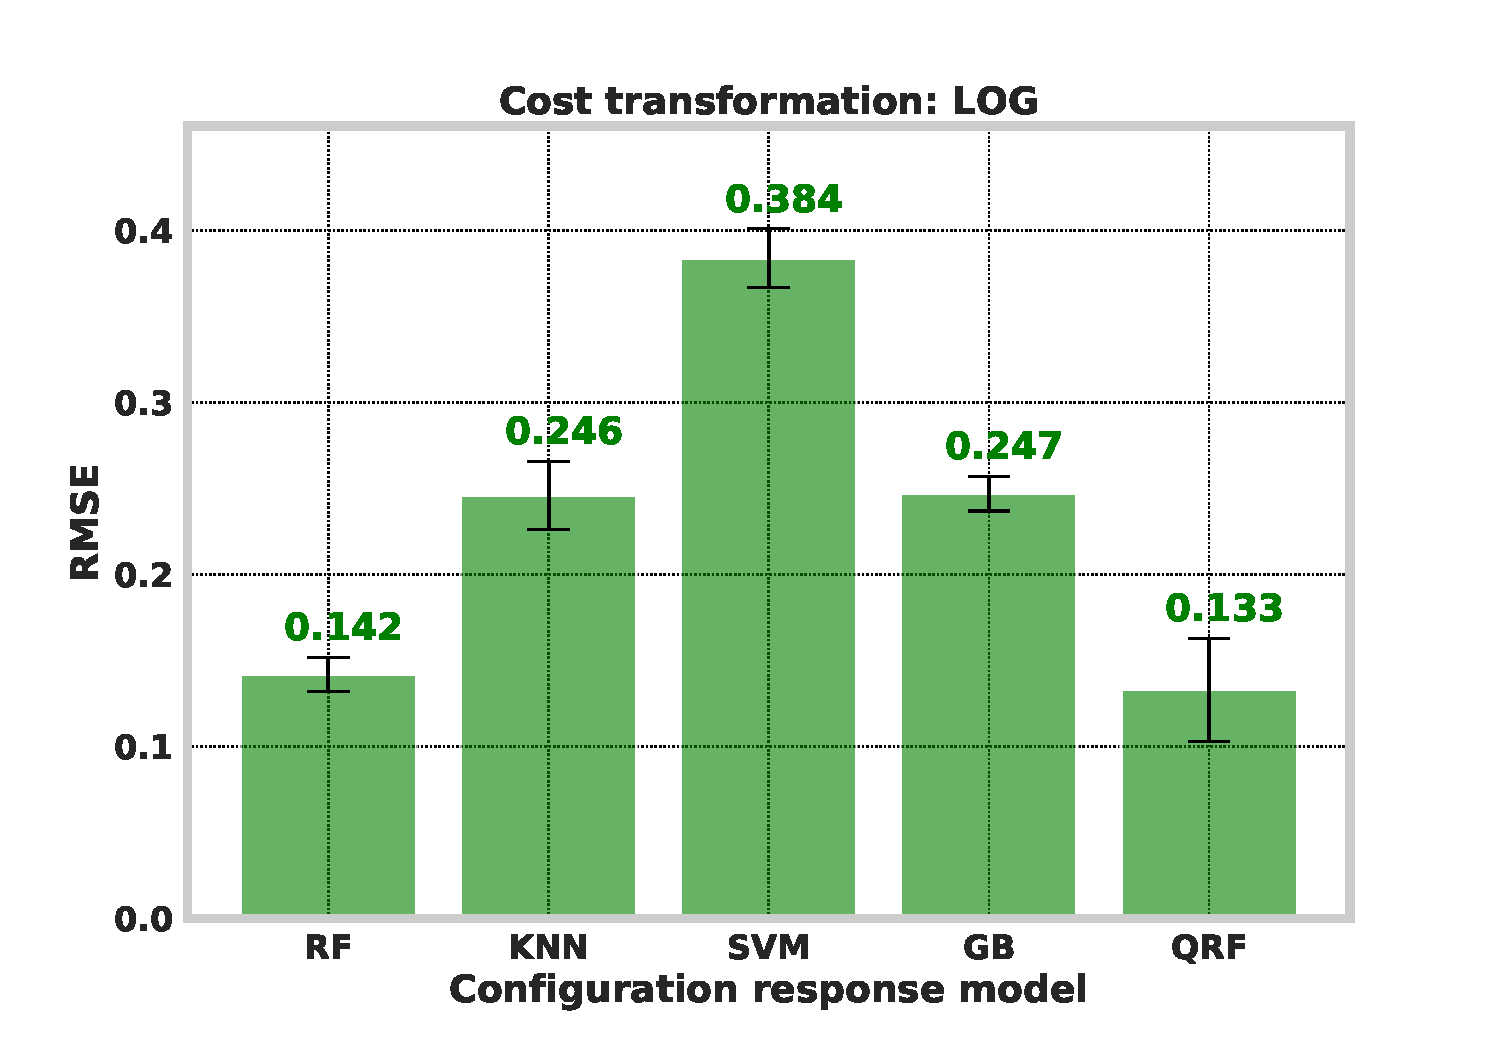
\includegraphics[width=\textwidth]{images/rmse-config_1.pdf}
              \caption{Rank 1}
        \end{subfigure}
        \begin{subfigure}{.47\textwidth}
              \centering
              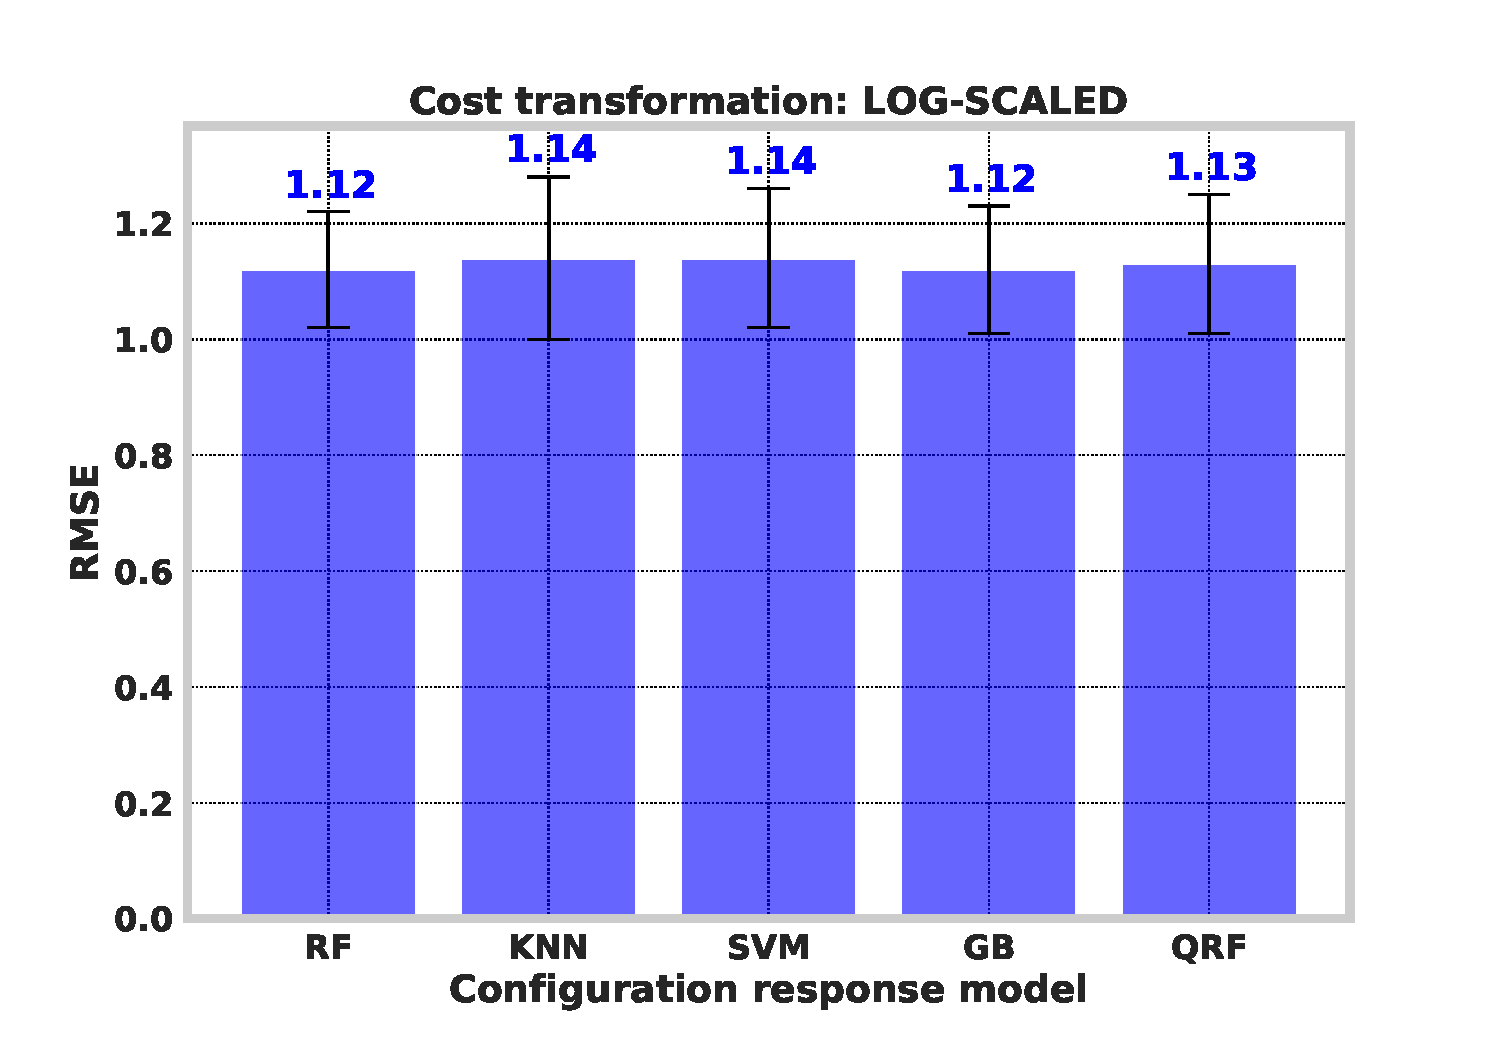
\includegraphics[width=\textwidth]{images/rmse-config_2.pdf}
              \caption{Rank 2}
        \end{subfigure}
        \begin{subfigure}{.47\textwidth}
              \centering
              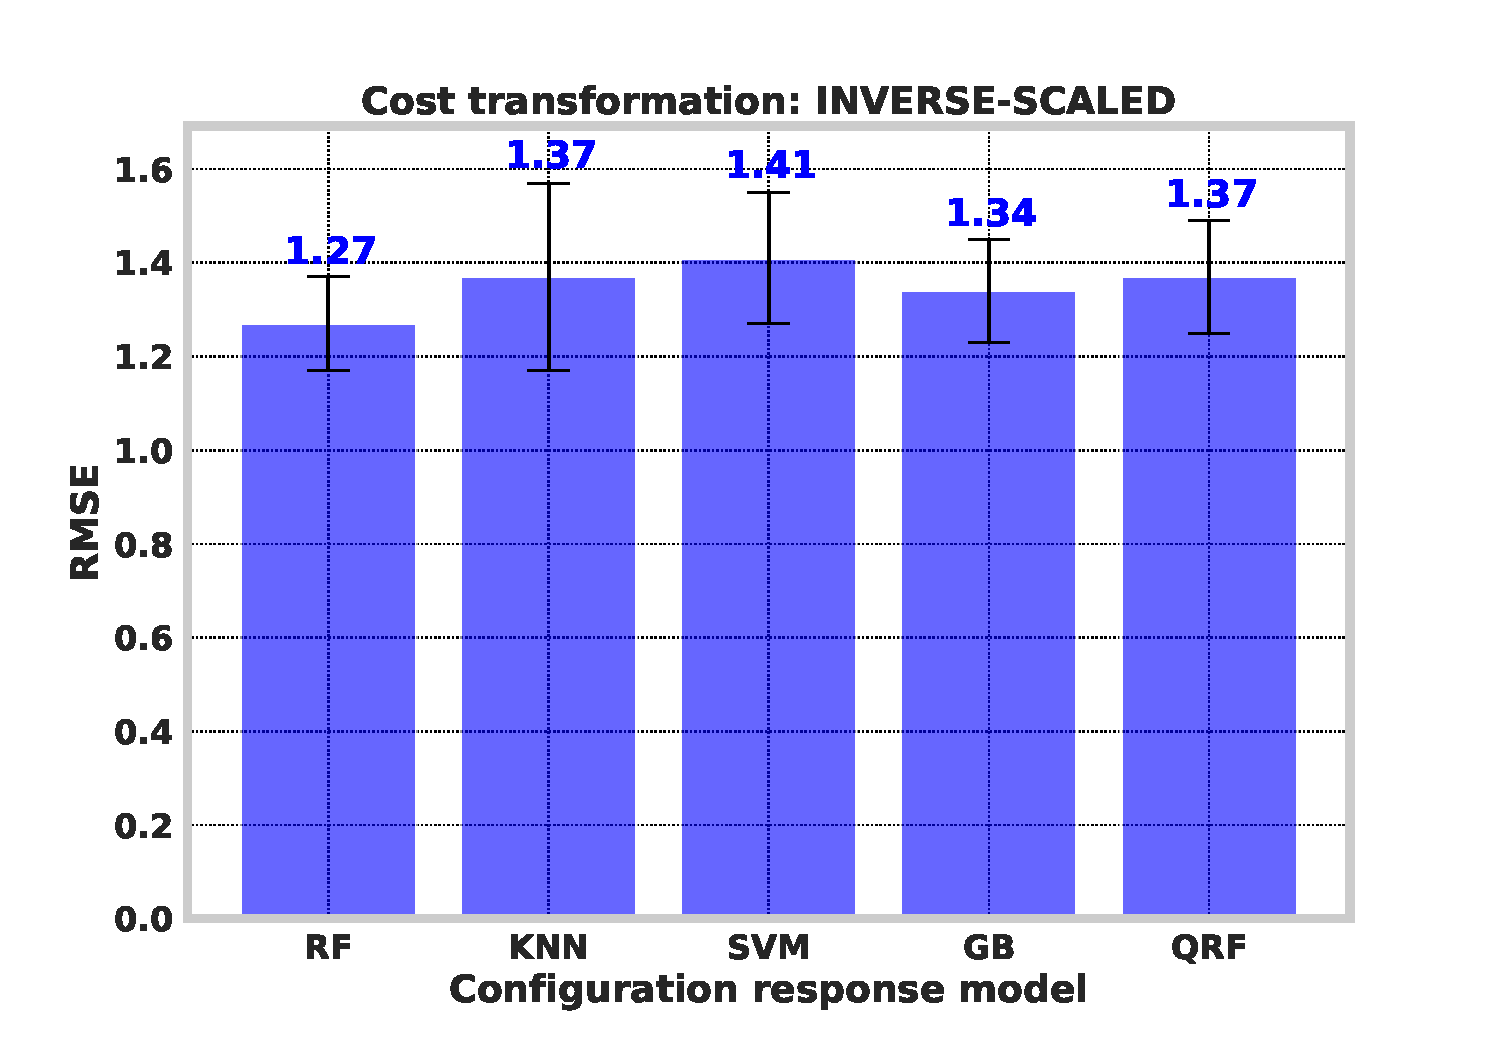
\includegraphics[width=\textwidth]{images/rmse-config_3.pdf}
              \caption{Rank 3}
          \end{subfigure}
          \begin{subfigure}{.47\textwidth}
              \centering
              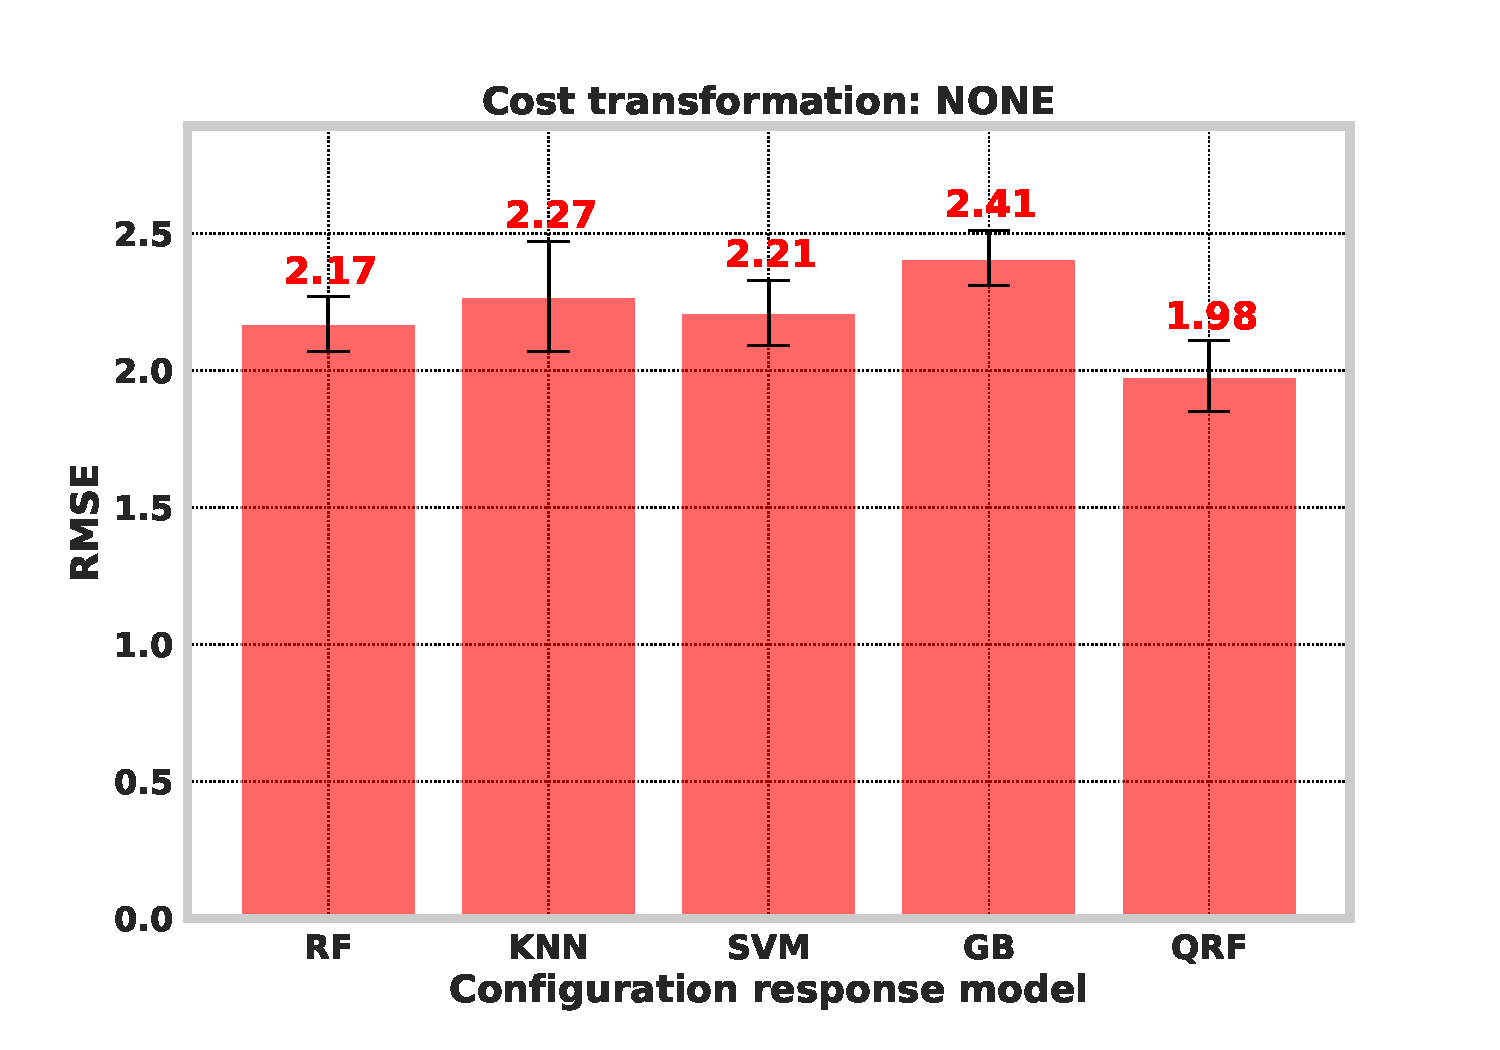
\includegraphics[width=\textwidth]{images/rmse-config_0.pdf}
              \caption{Rank 4}
            \end{subfigure}
\captionsetup{justification=justified}    
\caption[RMSE for configuration response models]{RMSE for different configuration response models using 5-fold CV.The green and red bars indicate the least and largest error, respectively, among the models for different transformations. The number on top of each bar is the mean RMSE of the model provided by 5-fold CV\footnotemark. The error bars (black lines with an upper and lower bound) is the deviation across 5-folds.}
\label{fig:config_response_result}
\end{figure}
\footnotetext{The RMSE values in each individual graph is rounded to same significant figures in a particular graph.}
}


\afterpage{
\begin{figure}[!h]
        \centering
        \begin{subfigure}{.47\textwidth}
              \centering
              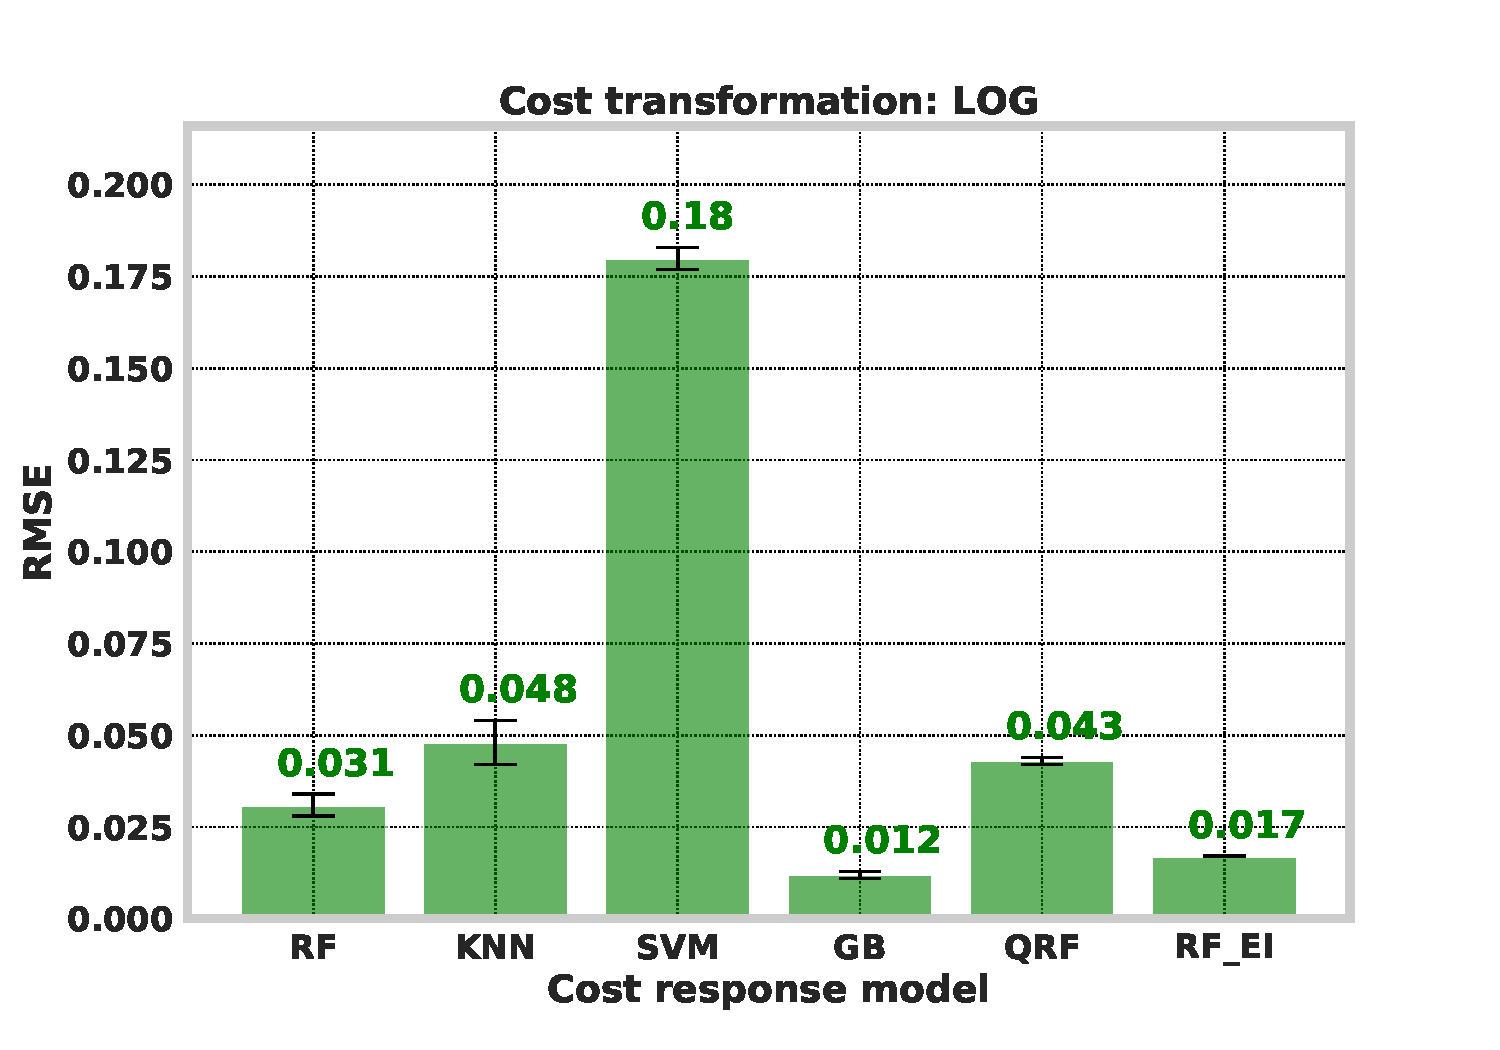
\includegraphics[width=\textwidth]{images/rmse-cost_1.pdf}
              \caption{Rank 1}
        \end{subfigure}
        \begin{subfigure}{.47\textwidth}
              \centering
              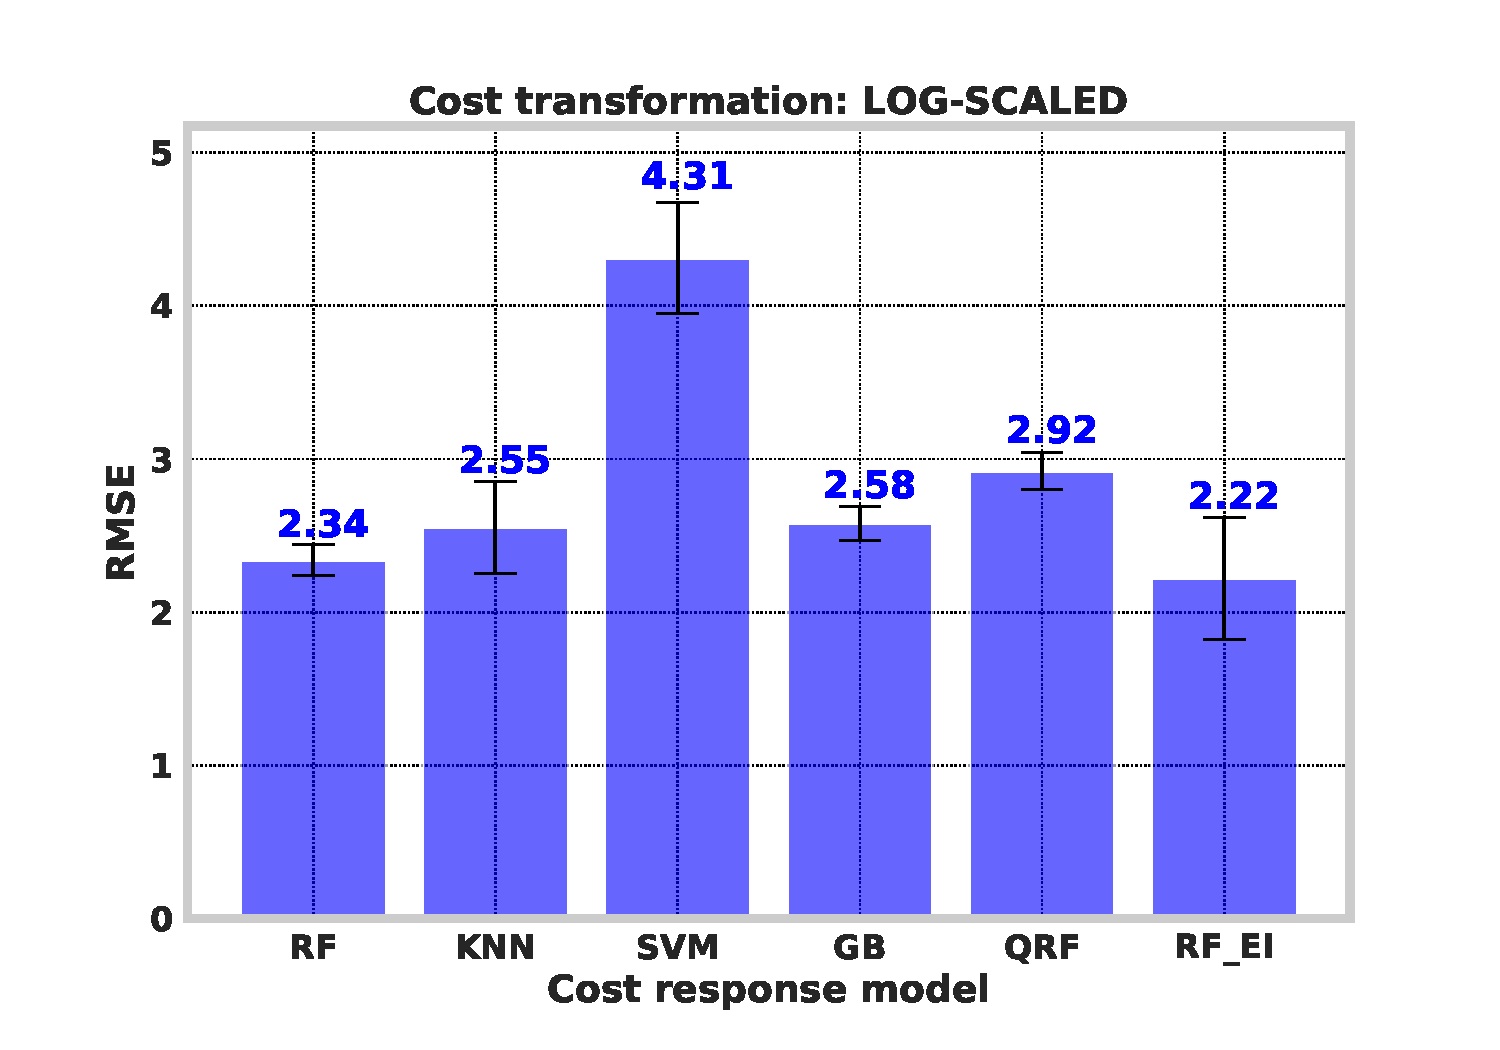
\includegraphics[width=\textwidth]{images/rmse-cost_2.pdf}
              \caption{Rank 2}
        \end{subfigure}
        \begin{subfigure}{.47\textwidth}
              \centering
              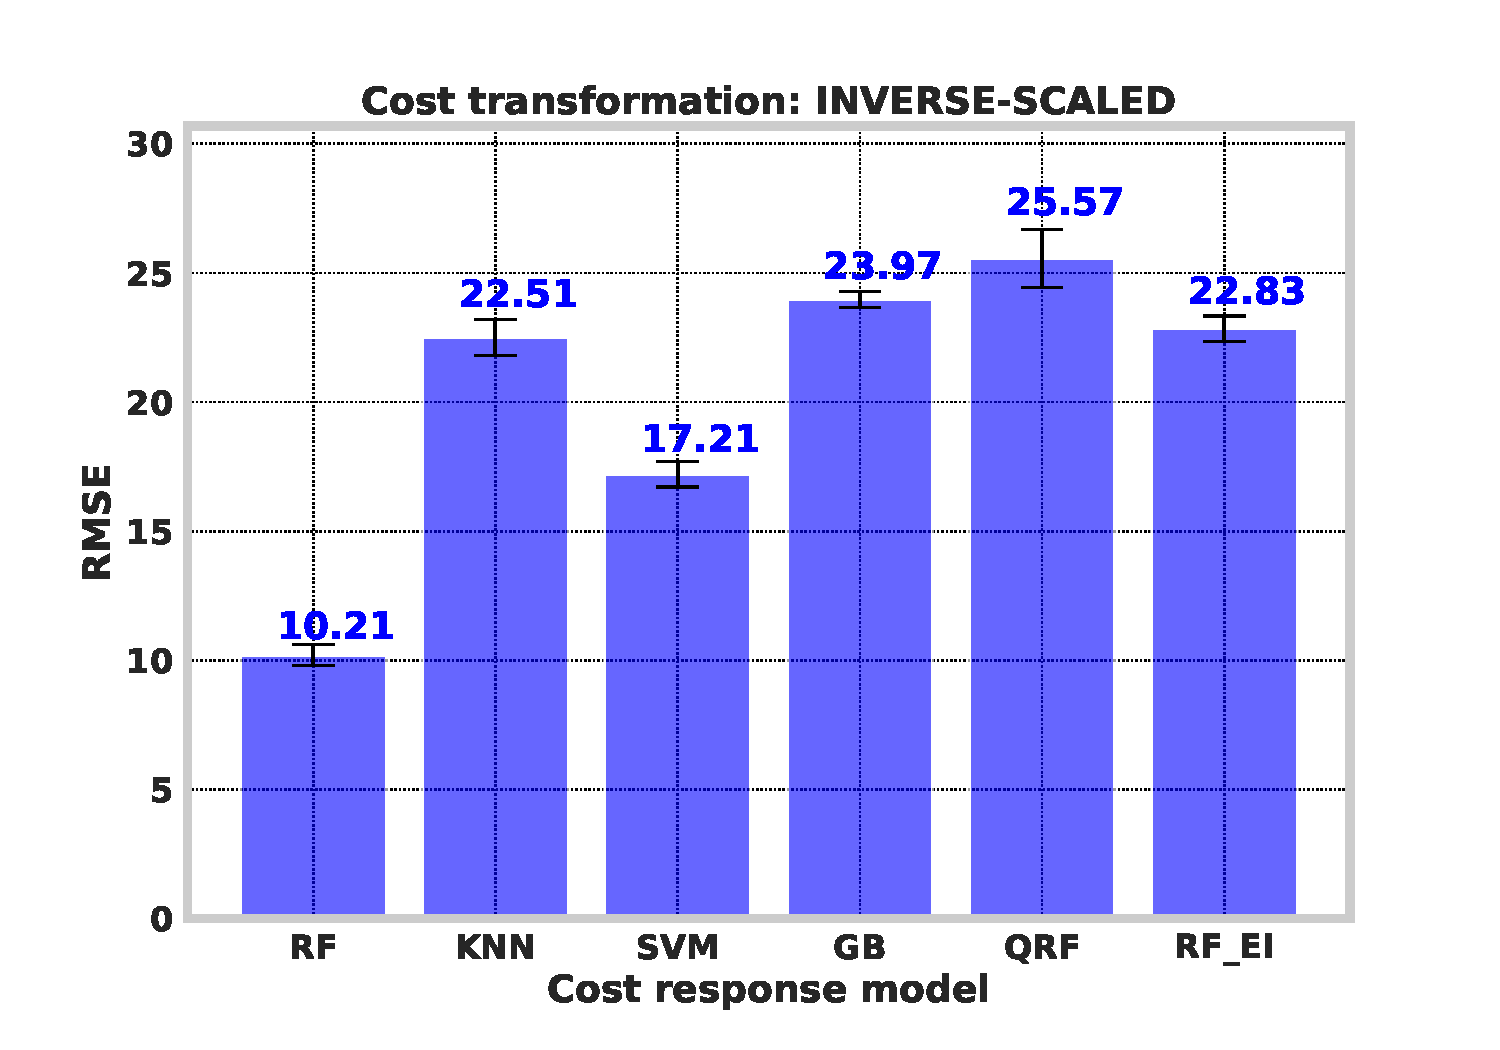
\includegraphics[width=\textwidth]{images/rmse-cost_3.pdf}
              \caption{Rank 3}
        \end{subfigure}
        \begin{subfigure}{.47\textwidth}
              \centering
              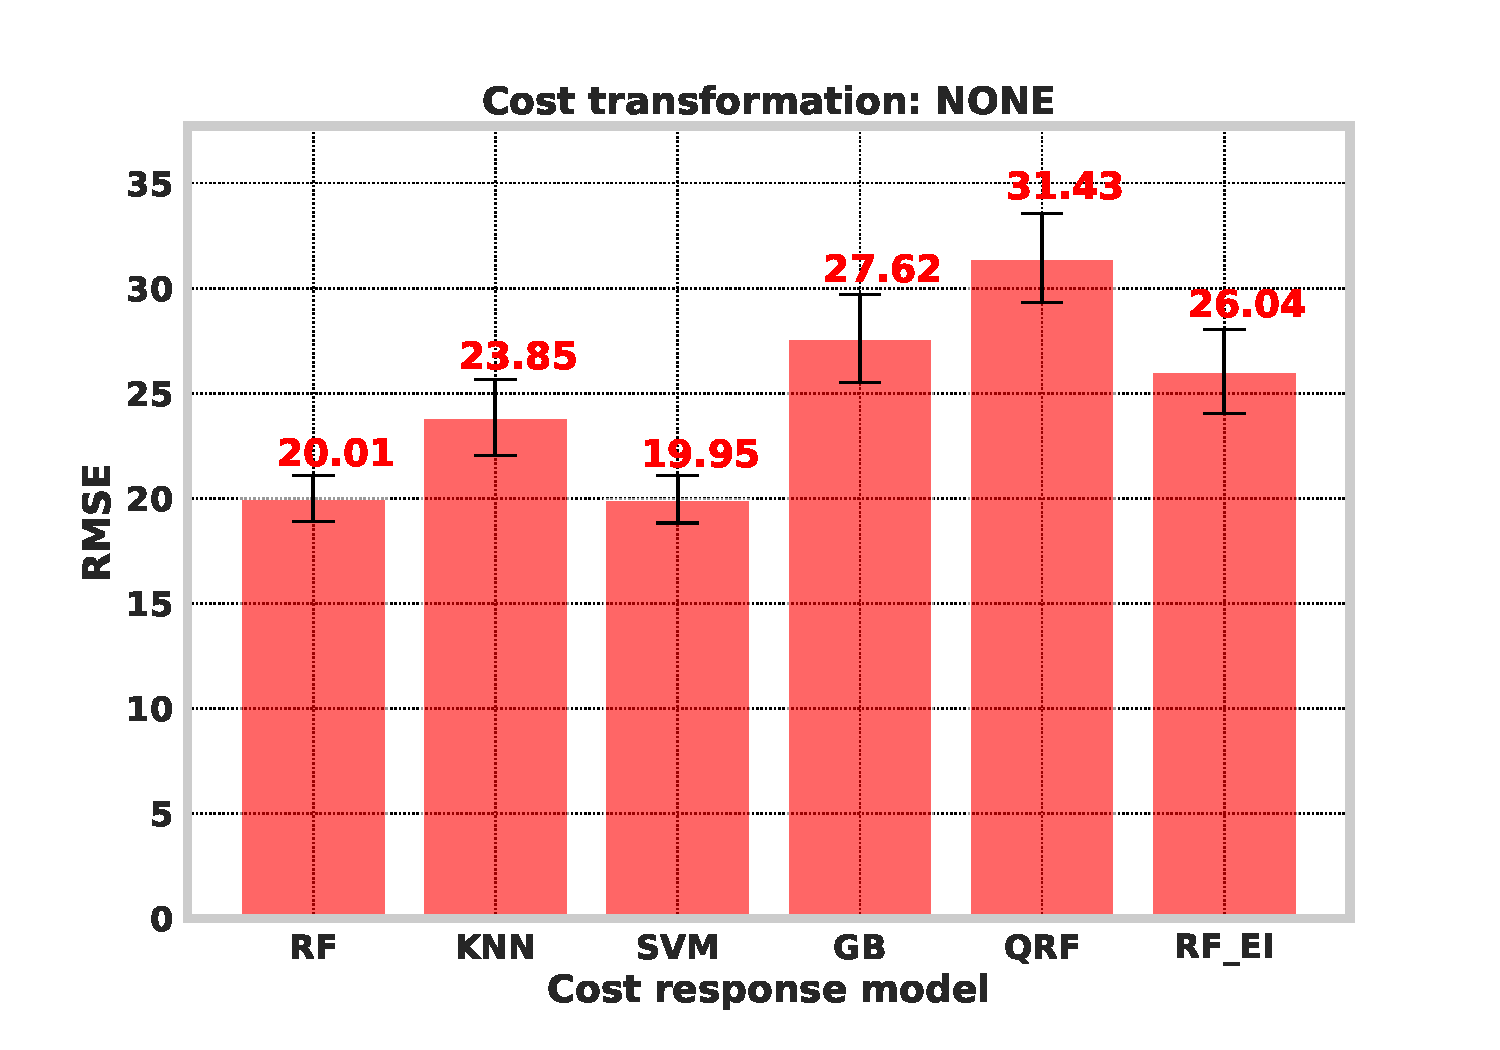
\includegraphics[width=\textwidth]{images/rmse-cost_0.pdf}
              \caption{Rank 4}
            \end{subfigure}
\captionsetup{justification=justified}
\caption[RMSE for cost response models]{RMSE for different cost response models using 5-fold CV. The green and red bars indicate the least and largest error, respectively, among the models for different transformations. The number on top of each bar is the mean RMSE of the model provided by 5-fold CV\footnotemark. The error bars (black lines with an upper and lower bound) is the deviation across 5-folds.}
\label{fig:cost_response_result}
\end{figure}
\footnotetext{The RMSE values in each individual graph is rounded to same significant figures in a particular graph.}
}

The log transformation of the runtime performs better than other transformations because it reduces the skewness and variances in the data. The skewness and standard deviation for all different types of transformed data are provided in table \ref{table:skewness}. The less spread in the predictor variable aids in better prediction and less RMSE in the model evaluation. The figures \ref{fig:config_response_result} and \ref{fig:cost_response_result} illustrate the importance of logarithmic transformation with less error model evaluation. \raggedbottom The various previous works on runtime prediction recommend logarithmic transformation of the runtime because logarithmic transformation aids in runtime prediction by reducing the dynamic range of the runtime \cite{SMAC_mainpaper} \cite{SMAC_extendedpaper}. 

The RMSE error of cost and configuration response models are incomparable. The cost response model errors are a dimensionless quantity (normalized cost), representing only the error in the cost variable. In contrast, the configuration response models illustrate the distance between the predicted response vector (vector of configurations) and the actual response vector. Furthermore, a small magnitude of error is tolerable in the cost response models. However, a small error in the configuration response model at worst case result in switching the category of the categorical parameters. In order to avoid such worst-case errors, models trained by logarithmic transformation is selected for evaluation on unseen simulation instances.

\begin{table}[!h]
\centering
\begin{tabular}{|l|l|l|}
\hline
\multicolumn{1}{|c|}{\multirow{2}{*}{\textbf{Transformation}}} & \multicolumn{2}{c|}{\textbf{Pre-processed cost metric}} \\ \cline{2-3} 
\multicolumn{1}{|c|}{} & \multicolumn{1}{c|}{\textbf{Skewness}} & \multicolumn{1}{c|}{\textbf{Standard deviation}} \\ \hline
LOG & \color{OliveGreen}0.2152 & \color{OliveGreen}0.6718\\ \hline
LOG-SCALED & -1.036 & 7.417 \\ \hline
INVERSE & -1.532 & 2501 \\ \hline
NONE & \color{red}\textbf{6.331} & \color{red}\textbf{3304} \\ \hline
\end{tabular}
\captionsetup{justification=justified}
\caption[Statistical measures of the pre-processed cost metrics]{Statistical measures of the pre-processed cost metrics using different transformations. The green and red highlights indicate the first and last ranked statistical values, respectively, across different transformations.}
\label{table:skewness}
\end{table}

\section{Evaluation of smart-coupling on an unseen simulation instance}
\label{section:real_eval}

The experimental setup provides the overview of the simulation instances used in evaluation. The evaluation metrics are defined in the following section \ref{section:evaluation_metrics}. In addition, the results illustrate the performance of the models.

\subsection{Experimental setup}
The evaluation is performed on two unseen simulation instances of 3D driven cavity. The machine learning models and the training dataset from SMAC have not seen the simulation instance features. In addition, the evaluation simulation instances cover critical cases with density ratio 1. The density ratio value 1 is critical from the computation point of view in the coupling tool \cite{criticalinstances}. The features of the evaluation simulation instances are provided in table \ref{table:simulationinstances_evaluation}. 

The two simulation instances are configured by the parameters predicted by the models trained using the logarithmically transformed cost values. A total of 11 configurations are predicted by the 6 cost response models and 5 configuration response models. This leads to 11 simulations of each instance with different parameters and a total of 22 simulations. OpenFOAM and Calculix are the fluid and solid solvers used in the simulation.

The model performance in the simulation instances is evaluated using the metric provided in the next section. 

\begin{table}[!ht]
\centering
\begin{tabular}{|l|l|}
\hline
Number of machine learning models & 11 \\ \hline
Number of evaluation simulation instances & 2 \\ \hline
Number of configurations predicted by each model & 1 \\ \hline
Transformations used for cost variable & LOG \\ \hline
Total evaluation simulation instances & 11 x 2 x 1 = 22 \\ \hline
\end{tabular}
\captionsetup{justification=justified}
\caption[Summary of evaluation simulation instances]{Summary of the number of evaluation simulation instances.}
\label{table:totalevaluation}
\end{table}

\subsection{Evaluation metrics}
\label{section:evaluation_metrics}
\subsubsection{Normalized Runtime (NR)}

NR  of a configuration obtained from 'X' is the ratio of the simulation runtime with the particular configuration obtained from 'X' to the simulation runtime of the best configuration for a particular simulation. 'X' can be a machine learning model or SMAC. NR is calculated for each configuration predicted by the model for a particular instance. NR less than 1 illustrates a better performance of the configuration predicted by the model relative to the best configuration runtime. The best configuration is the configuration obtained from SMAC.  Therefore, NR for the best configuration from SMAC is 1, i.e., 'X' is SMAC. 

\begin{equation}
\text{NR of a configuration from 'X'} = \frac{\text{Runtime of the configuration from 'X'}}{\text{Runtime of the best configuration from SMAC}}   
\label{equation:normalized}
\end{equation}

\subsubsection{Average Normalized Runtime (ANR)}

ANR of configurations obtained from 'X' provides a measure of the performance of 'X' over a set of simulation instances. Similar to NR, 'X' can be a machine learning or SMAC. The ANR of the configuration obtained from model 'X' is the average of the NR obtained from the model for all the simulation instances in the evaluation set.  ANR for the best configurations from SMAC is 1.

\begin{equation}
\begin{split}
\text{ANR of configurations from 'X'} = \frac{\Sigma_{i=1}^{N} \text{{NR of a configuration from 'X' on instane i}}}{N}
\label{equation:averagenormalized}
\end{split}
\end{equation}

% Should be changed to benchmark runtime from SMAC optimization.
% Average normalized default runtime
% Normalized runtime
NR of a configuration from a particular model is given in equation \ref{equation:normalized}. In equation \ref{equation:averagenormalized}, model 'X' is the cost or configuration response model, $i$ is a particular simulation instance, and $N$ is the total number of simulation instances in the evaluation set.

\subsection{Results and discussion}

The figure \ref{fig:final_eval} illustrates the performance of models selected from the previous experiment on unseen simulation instances. The RF model predicting each parameter of the configuration by regression is performing better compared to the other configuration response models because RF handles categorical parameters better \cite{Hutterphd}. In contrast, the random forest predicting the expected improvement metric is performing better in the cost response model. This illustrates the performance of the models in two simulation instances.

\begin{figure}[!ht]
\centering
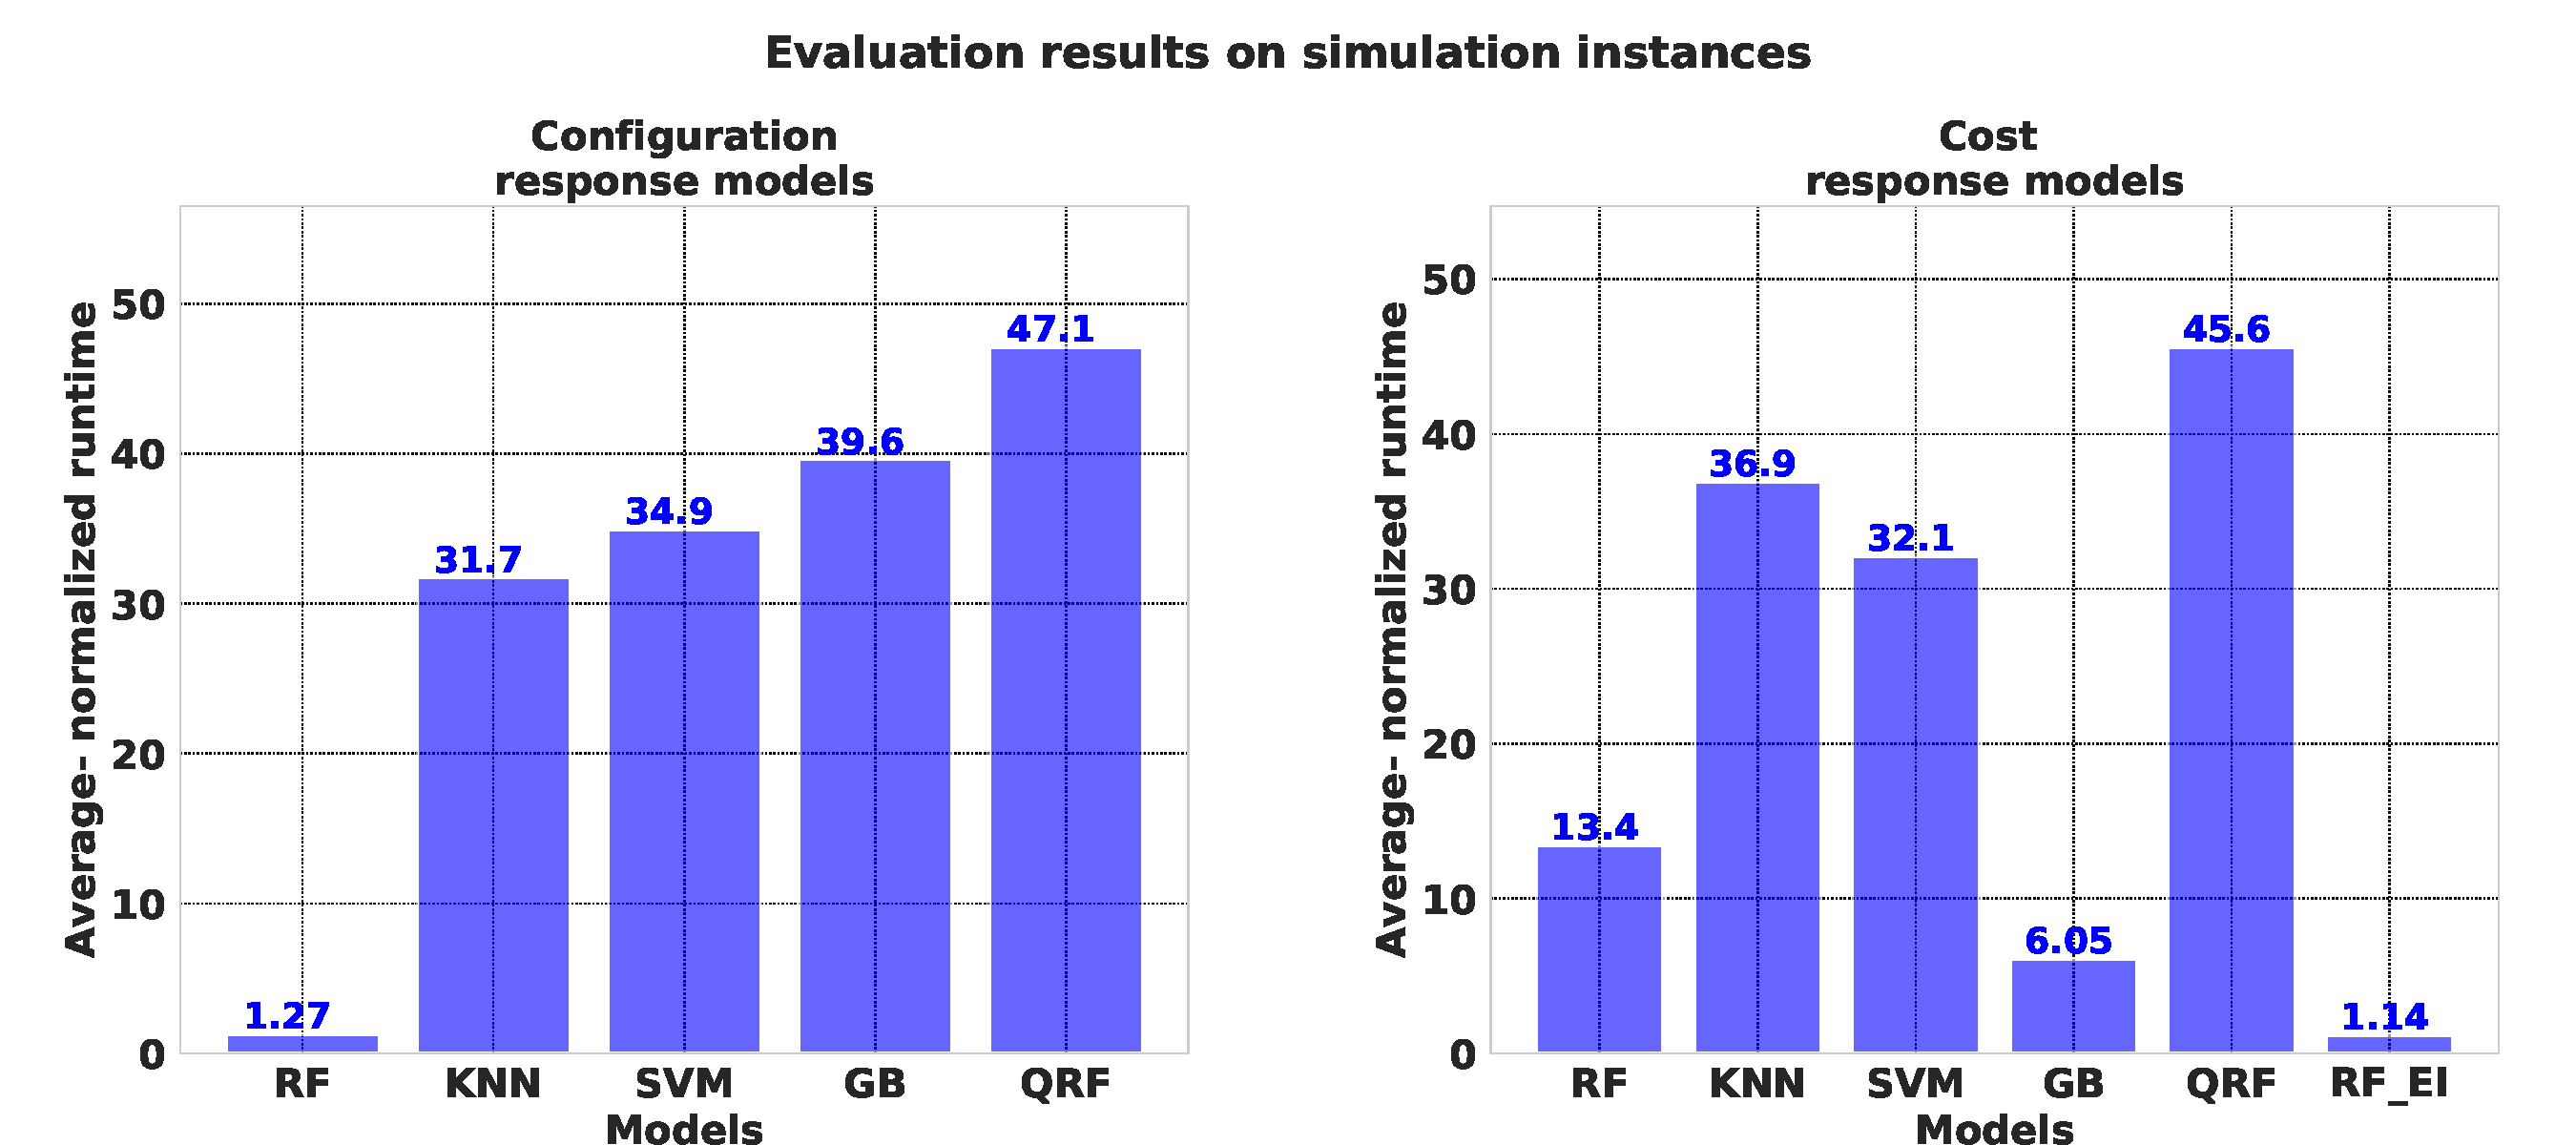
\includegraphics[width=\textwidth]{images/final-eval.pdf}
\captionsetup{justification=justified}
\caption[Configuration and cost response models evaluation results]{Configuration and cost response model evaluation results on simulation. The lower value is the better model.}
\label{fig:final_eval}
\end{figure}

On looking closer into the ANR metric, the runtime of each configuration predicted by a model is normalized using the runtime of the best configuration from the optimization of a particular instance using SMAC. The runtime of the best configuration from SMAC is the benchmark runtime for each instance. Therefore, the average normalized runtime of the best configuration from SMAC\footnote{NR of the best configuration from SMAC for a particular simulation instance is 1. Therefore, the ANR across the set of evaluation instances is 1.} for a particular instance is 1.

The model with an ANR less than 1, perform better than the best configuration of SMAC. However, the models cannot predict configurations better than the best configuration from SMAC. The reason is the configurations from SMAC are obtained by performing per-instance optimization of the simulation instance over 100 evaluations of the target algorithm, MpCCI. 

 The top three models are suggested to the user. The selection criteria is the models with an order of magnitude, 1, from the average normalized runtime of the best cost. In addition, all the models are performing better than the default configuration.

In figure \ref{fig:real_eval}, the default configuration results in a crashed simulation. However, the performance of the top 3 models is extremely helpful in meeting the desired result of the research work.

\begin{figure}[!ht]
\centering
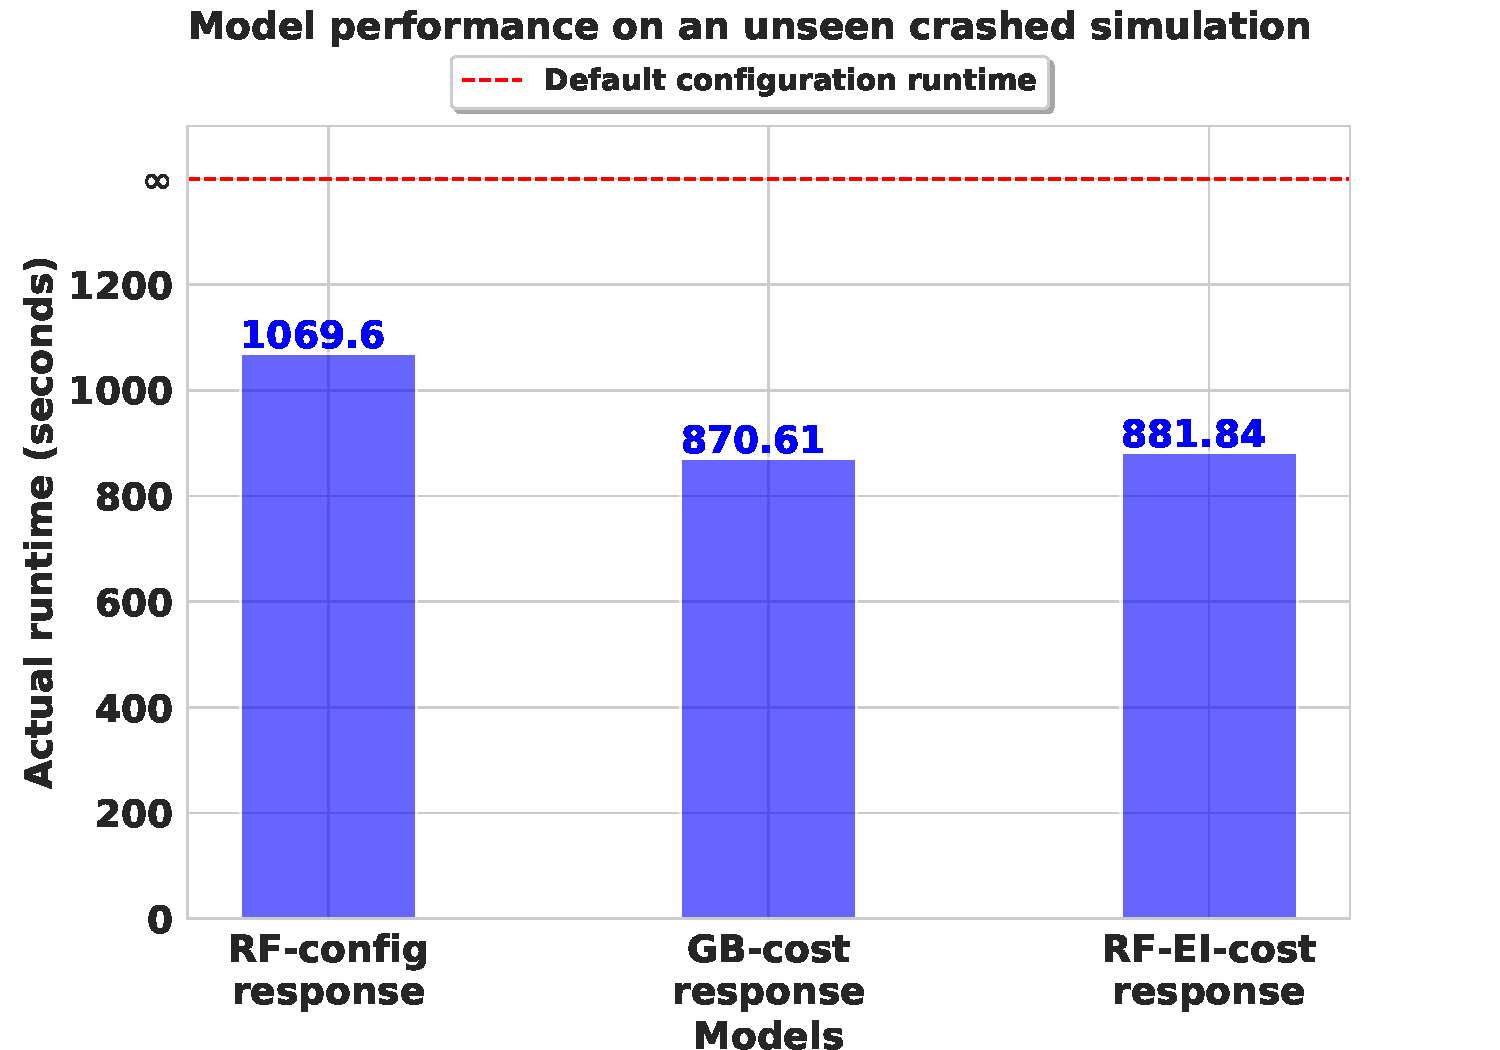
\includegraphics[width=\textwidth]{images/real-eval.pdf}
\captionsetup{justification=justified}
\caption[Model performance on a critical unseen simulation instance]{Model performance on a critical simulation instance (solid-to-fluid density ratio is 1).}
\label{fig:real_eval}
\end{figure}

% https://www.calculatorsoup.com/calculators/math/significant-figures-rounding.php


\section{Summary}

The chapter addresses the different experiments conducted to evaluate the smart coupling tool developed. The summary of the main observations from the experiments is provided below.  
\begin{enumerate}

\item  A single simulation instance with a particular feature set is optimized using SMAC. The SMAC best configuration provides a lesser runtime compared to the default configurations of MpCCI. SMAC successfully estimates a configuration better than the default configuration with a win-percentage of 100\%. In addition, SMAC provides a mean decrease in runtime of approximately 25\%. This aids in developing a dataset with configurations better than the default configuration. The dataset is used for training models to predict a configuration with lesser runtime provided an unseen simulation instance.

\item One of the imperative aspects of SMAC is the ability to find a better configuration on a crashed simulation instance for the default configuration. On all 4 crashed simulation instances with default configurations, SMAC is able to estimate a better configuration successfully. 

%----- Less important point Discuss ------
\item Currently, all the configurations resulting in a successful simulation are considered for building a machine learning model to predict better configurations. However, the choice between selecting all the good configurations and only the best configuration for a simulation instance should be explored in the future. 

\item The repeatability of SMAC in optimizing a multiphysics simulation is evaluated in section \ref{section:repeatability}. This aids in understanding the ability of SMAC to find good configurations with similar performance repeatedly. In addition, the variance associated with the performance of the configurations generated from SMAC is illustrated. The repeatability coefficient of SMAC is 19.34 seconds.

\item The relationship between the number of times SMAC evaluates the objective function, and the performance of the best configuration from SMAC is directly proportional. The larger the number of times a target algorithm is evaluated, SMAC finds configurations with better performance. However, to effectively manage the resources and reduce the number of target algorithm evaluations, SMAC runs the target algorithm for 100 iterations.

\item On analyzing the run history of SMAC, the number of bad configurations resulting in crashed simulation is approximately equal to the good configurations resulting in successful simulation within the 100 iterations of SMAC. The good configurations are important for the training of the model, and bad configurations are unimportant, leading to wastage of resources.

% \item One of the recommendations to reduce the number of bad configuration evaluations by SMAC is to prune SMAC by a classifier model. The classifier model classifies the successful and crash simulation for a particular parameter configuration and feature set of the simulation. The classifier model selection is made by 5-fold cross-validation. SVM outperforms RF, GB, KNN, and logistic regression in terms of accuracy, precision, recall, and F1 score.

\item The regression models to predict the best configuration given a simulation instance is trained in two methods, namely cost and configuration response models. In addition, the cost feature (runtime in seconds) of a particular simulation instance is transformed in 4 different ways, namely logarithmic, scaled-logarithmic, scaled-inverse, and none. The model selection incorporates the 5-fold cross-validation technique. The models illustrate relatively better performance on logarithm transformed cost metric with less RMSE. All the models are trained on the complete data available with logarithm transformed cost features for real-time evaluation on unseen simulation instances. 

\item To evaluate the model performance on the unseen instance, an Average Normalized Runtime (ANR) metric is devised. After evaluating all the models trained with logarithm transformed cost, the top three models are selected for integration to the smart coupling tool. In figure \ref{fig:final_eval}, the predicted configurations for each evaluation instance is compared against the best cost obtained by optimizing each evaluation instance. This best cost is treated as a benchmark. The predicted configurations are not performing better than the best cost because the best cost is obtained by optimizing each instance for 100 iterations using SMAC. Therefore, the top three models performing close to the best cost are suggested to the user by the smart coupling tool.

\item On comparing the actual runtime of the suggested parameter configuration against the default configurations runtime in figure \ref{fig:real_eval}, the model performance is effective than the default. This illustrates the effectiveness of the smart coupling tool to estimate an optimal configuration for a simulation that crashed with the default configurations.

\item The configurations from RF- configuration response model, GB- cost response model, and RF predicting expected improvement are reliable, providing relatively less runtime than other models. The time taken by the smart coupling tool to suggest the three configurations is 0.621 seconds. 

\end{enumerate}

